\chapter{Richtlinien zu Forschungsdaten aus deutschen Promotionsvorhaben}\label{ch:richtlinien}

\parsum{Thema des Kapitels}
Dieses Kapitel behandelt die verschiedenen verwaltungsrechtlichen Dokumente wissenschaftlicher Institutionen, die ein Promotionsvorhaben in Bezug auf \gls{fdm} entweder spezifisch oder auch nur allgemein betreffen.
Es wird überprüft, inwiefern promotionsberechtigte Institutionen in Deutschland bereits derlei Richtlinien erlassen haben, in welcher Form diese existieren und welche Anforderungen diese stellen.

\parsum{Aufbau des Kapitels}
Hierfür wird in \cref{sec:policy-material-methods} aufgeführt, wie die zu untersuchenden Institutionen ausgewählt wurden, wie welche Materialien der Institutionen ausgesucht wurden und mit welchen Methoden das gesammelte Material daraufhin ausgewertet wurde.
In \cref{sec:policy-results} werden die entsprechenden Ergebnisse der Materialauswertung dargestellt.
Abschließend werden in \cref{sec:policy-discussion} die dargestellten Ergebnisse evaluiert und diskutiert.

\section{Material \&\ Methoden}\label{sec:policy-material-methods}
\parsum{Aufbau des Abschnitts}
In diesem Abschnitt wird das zu untersuchende Material in \cref{sec:policy-material} und die Methoden der Untersuchung in \cref{sec:policy-methods} dargestellt.

\subsection{Material}\label{sec:policy-material}
\parsum{Datengrundlage}
Da es in Deutschland hierzu keine offizielle und öffentlich zugängliche Liste aller Universitäten mit Promotionsrecht seitens des Bundesministeriums für Bildung gibt, wird als Datengrundlage für dieses Kapitel die von der \citeauthor{Hochschulkompass-Liste} geführte Liste aller wissenschaftlichen Institutionen aus dem tertiären Bildungsbereich in Deutschland \autocite{Hochschulkompass-Liste} genutzt.
Diese Liste wird tagesaktuell geführt, basiert auf der Selbstauskunft aller involvierten Institutionen ($n=428$), kodifiziert unter anderem welche Institutionen das Promotions- und Habilationsrecht führen, umfasst auch Institutionen, die nicht Mitglied der \citeauthor{Hochschulkompass-Liste} sind und besitzt einen \textit{de facto} wenn auch nicht \textit{de jure} Status als Datengrundlage für allgemeine Informationen zu wissenschaftlichen Institutionen aus Deutschland. Für die tagesspezifische Version der Liste, die für diese Arbeit genutzt wurde, siehe \fxfatal*{ADD LINK TO DIGITAL APPENDIX!}{FIXME!}.

\parsum{Grundmengenbeschreibung}
Um die zentrale Forschungsfrage dieses Kapitels zu beantworten, wurde diese Liste auf nur jene Institutionen gefiltert, welche das Promotionsrecht besitzen ($n=163$).
Die resultierende Liste promotionsberechtigter Institutionen besteht aus Forschungsinstutionen verschiedener Hochschultypen sowie unterschiedlicher Trägerschaften.
Von den Hochschultypen her umfasst die Liste Universitäten, \glspl{fh}, \glspl{haw}, \glspl{kh}, eine \gls{vh} sowie eine \gls{hset}.
Von den Trägerschaften her umfasst die Liste öffentlich-rechtliche, private sowie kirchliche Institutionen. Alle Institutionen sind staatlich anerkannt.
Die relative sowie die absolute Distribution aller promotionsberechtigter Institutionen in Deutschland nach Hochschultyp und Trägerschaft ist in \cref{tab:grundmenge-beschreibung-art} gegeben.
\begin{table}[!htbp]
	\caption{Die Verteilung aller promotionsberechtigter Institutionen in Deutschland nach $\text{\textit{Hochschultyp}}\times\text{\textit{Trägerschaft}}$ aufgegliedert. Absolute Werte in Klammern angegeben.}
    \resizebox{\ifdim\width>\textwidth\textwidth\else\width\fi}{!}{%
        \begin{tabular}{lS[table-format=3.2]@{\,}S[table-text-alignment = left]lS[table-format=3.2]@{\,}S[table-text-alignment = left]lS[table-format=3.2]@{\,}S[table-text-alignment = left]lS[table-format=3.2]@{\,}S[table-text-alignment = left]l}
            \toprule
            & \multicolumn{3}{c}{\textbf{Öffentlich-Rechtlich}} & \multicolumn{3}{c}{\textbf{Privat}} & \multicolumn{3}{c}{\textbf{Kirchlich}} & \multicolumn{3}{c}{\textbf{Summe}}    \\
            \midrule
            \textbf{Universität}  & 53,37 & \si{\percent} & (87)  & 7,98 & \si{\percent} & (13) & 6,13 & \si{\percent} & (10) & 67,48  & \si{\percent} & (110) \\
            \textbf{\gls{fh} / \gls{haw}}     & 6,75  & \si{\percent} & (11)  & 0,00 & \si{\percent} & (0)  & 0,00 & \si{\percent} & (0)  & 6,75   & \si{\percent} & (11)  \\
            \textbf{\gls{kh}}          & 23,93 & \si{\percent} & (39)  & 0,61 & \si{\percent} & (1)  & 0,00 & \si{\percent} & (0)  & 24,54  & \si{\percent} & (40)  \\
            \textbf{\gls{hset}}         & 0,61  & \si{\percent} & (1)   & 0,00 & \si{\percent} & (0)  & 0,00 & \si{\percent} & (0)  & 0,61   & \si{\percent} & (1)   \\
            \textbf{\gls{vh}}          & 0,61  & \si{\percent} & (1)   & 0,00 & \si{\percent} & (0)  & 0,00 & \si{\percent} & (0)  & 0,61   & \si{\percent} & (1)   \\\midrule
            \textbf{Summe}        & 85,28 & \si{\percent} & (139) & 8,59 & \si{\percent} & (14) & 6,13 & \si{\percent} & (10) & 100,00 & \si{\percent} & (163) \\
            \bottomrule
        \end{tabular}
    }
	\label{tab:grundmenge-beschreibung-art}
\end{table}

\noindent Geografisch gesehen sind, in der gefilterten Liste, zu unterschiedlich hohen Anteilen, Institutionen aus allen deutschen Bundesländern vertreten.
Die genaue Verteilung ist in \cref{fig:DE-grundmenge-beschreibung} wiedergegeben.
\begin{figure}[!htbp]
    \centering
    \begin{tikzpicture}[y=1cm, x=1cm, yscale=.8,xscale=.8, every node/.append style={scale=1}, inner sep=0pt, outer sep=0pt]
  \footnotesize
  \drawgermany
  \drawbw{colorblindC1!93}{25}
  \drawbav{colorblindC1!78}{21}
  \drawbrandenburg{colorblindC1!15}{4}
  \drawhessen{colorblindC1!59}{16}
  \drawmecklenburg{colorblindC1!11}{3}
  \drawniedersachsen{colorblindC1!48}{13}
  \drawnrw{colorblindC1!100}{27}
  \drawrheinland{colorblindC1!30}{8}
  \drawsaarland{colorblindC1!11}{3}
  \drawsachsen{colorblindC1!33}{9}
  \drawsachsenanhalt{colorblindC1!26}{7}
  \drawschleswig{colorblindC1!19}{5}
  \drawthuringen{colorblindC1!19}{5}
  \drawbremen{colorblindC1!7}{2}
  \drawhamburg{colorblindC1!30}{8}
  \drawberlin{colorblindC1!26}{7}
\end{tikzpicture}
    \caption{Die absolute Anzahl promotionsberechtigter Institutionen nach Bundesland.}
    \label{fig:DE-grundmenge-beschreibung}
\end{figure}

\noindent Für die gesamte Liste promotionsberechtigter Institutionen, siehe \fxfatal*{ADD LINK TO DIGITAL APPENDIX!}{FIXME!}

\parsum{Stichprobenziehung}
Diese Liste promotionsberechtigter Institutionen bildete die Grundmenge für die Ziehung einer einfachen Zufallsstichprobe.
Bei der Auswahl der Stichprobe wurde ein Konfidenzintervall von \SI{95}{\percent} und eine Fehlerspanne von \SI{5}{\percent} zugrunde gelegt.
Diese Parameter gewährleisten, dass die Ergebnisse der Stichprobe mit hoher Wahrscheinlichkeit repräsentativ für die gesamte Population sind und die Unsicherheit der Schätzungen innerhalb akzeptabler Grenzen bleibt.
Um den Prozess der Stichprobenziehung zu automatisieren und eine zufällige Auswahl zu gewährleisten, wurde eine auf Python basierende Software \autocite{Krassnig2024-csv} genutzt, welche im Rahmen dieser Arbeit geschrieben wurde.%
\footnote{%
Die Software von \citeauthor{Krassnig2024-csv} \autocite{Krassnig2024-csv} nutzt standardmäßig die Anzahl an Nanosekunden seit dem Beginn der System-Epoche (1970-01-01T00:00:00Z) als Startwert für die Zufallsfunktion.
Der genutzte Startwert wird als begleitendes Metadatum der Stichprobe abgespeichert.
Die Ziehung ist somit wiederholbar und das Datum der Ziehung verifizierbar.} 

\parsum{Stichprobenbeschreibung}
Die so gezogene Stichprobe ($n=115$) besteht aus ca. \SI{71}{\percent} aller promotionsberechtigter Institutionen.
Die Stichprobe umfasst Institutionen aller Trägerschaften aus der Grundmenge: öffentlich-rechtliche, private sowie kirchliche Institutionen.
Darüber hinaus umfasst die Stichprobe von den Hochschultypen her Universitäten, \glspl{fh}, \glspl{haw} und eine \gls{hset}.
In der Stichprobe befindet sich nicht die \gls{vh}, die sich in der Grundmenge befindet.
Mit dieser Ausnahme sind somit alle anderen Hochschultypen vertreten.
Die relative sowie die absolute Distribution aller Institutionen in der Stichprobe nach Hochschultyp und Trägerschaft ist in \cref{tab:stichprobe-beschreibung-art} gegeben.
\begin{table}[!htbp]
	\caption{Die Verteilung der Institutionen in der Stichprobe nach $\text{\textit{Hochschultyp}}\times\text{\textit{Trägerschaft}}$ aufgegliedert. Absolute Werte in Klammern angegeben.}
    \resizebox{\ifdim\width>\textwidth\textwidth\else\width\fi}{!}{%
        \begin{tabular}{lS[table-format=3.2]@{\,}S[table-text-alignment = left]lS[table-format=3.2]@{\,}S[table-text-alignment = left]lS[table-format=3.2]@{\,}S[table-text-alignment = left]lS[table-format=3.2]@{\,}S[table-text-alignment = left]l}
            \toprule
            & \multicolumn{3}{c}{\textbf{Öffentlich-Rechtlich}} & \multicolumn{3}{c}{\textbf{Privat}} & \multicolumn{3}{c}{\textbf{Kirchlich}} & \multicolumn{3}{c}{\textbf{Summe}}    \\
            \midrule
            \textbf{Universität}  & 55,65 & \si{\percent} & (64)  & 8,70 & \si{\percent} & (10) & 4,35 & \si{\percent} & (5) & 68,70  & \si{\percent} & (79) \\
            \textbf{\gls{fh} / \gls{haw}}     & 6,96  & \si{\percent} & (8)  & 0,00 & \si{\percent} & (0)  & 0,00 & \si{\percent} & (0)  & 6,96   & \si{\percent} & (8)  \\
            \textbf{\gls{kh}}          & 22,61 & \si{\percent} & (26)  & 0,87 & \si{\percent} & (1)  & 0,00 & \si{\percent} & (0)  & 23,48  & \si{\percent} & (27)  \\
            \textbf{\gls{hset}}         & 0,87  & \si{\percent} & (1)   & 0,00 & \si{\percent} & (0)  & 0,00 & \si{\percent} & (0)  & 0,87   & \si{\percent} & (1)   \\
            \textbf{\gls{vh}}          & 0,00  & \si{\percent} & (0)   & 0,00 & \si{\percent} & (0)  & 0,00 & \si{\percent} & (0)  & 0,00   & \si{\percent} & (0)   \\\midrule
            \textbf{Summe}        & 86,09 & \si{\percent} & (99) & 9,57 & \si{\percent} & (11) & 4,35 & \si{\percent} & (5) & 100,00 & \si{\percent} & (115) \\
            \bottomrule
        \end{tabular}
    }
	\label{tab:stichprobe-beschreibung-art}
\end{table}

\noindent Geografisch gesehen sind, in der Stichprobe, zu unterschiedlich hohen Anteilen, Institutionen aus allen deutschen Bundesländern vertreten.
Die genaue Verteilung ist in \cref{fig:DE-stichprobe-beschreibung} wiedergegeben.
\begin{figure}[!htbp]
    \centering
    \begin{tikzpicture}[y=1cm, x=1cm, yscale=.8,xscale=.8, every node/.append style={scale=1}, inner sep=0pt, outer sep=0pt]
  \node[text=black,line width=0.0092cm,anchor=west] (title1) at (0,7){\textbf{(A)}};
  \footnotesize
  \drawgermany
  \drawbw{colorblindC1!77}{17}
  \drawbav{colorblindC1!55}{12}
  \drawbrandenburg{colorblindC1!18}{4}
  \drawhessen{colorblindC1!45}{10}
  \drawmecklenburg{colorblindC1!9}{2}
  \drawniedersachsen{colorblindC1!50}{11}
  \drawnrw{colorblindC1!100}{22}
  \drawrheinland{colorblindC1!23}{5}
  \drawsaarland{colorblindC1!9}{2}
  \drawsachsen{colorblindC1!23}{5}
  \drawsachsenanhalt{colorblindC1!27}{6}
  \drawschleswig{colorblindC1!9}{2}
  \drawthuringen{colorblindC1!9}{2}
  \drawbremen{colorblindC1!9}{2}
  \drawhamburg{colorblindC1!36}{8}
  \drawberlin{colorblindC1!23}{5}
\end{tikzpicture}\hfill%
\begin{tikzpicture}[y=1cm, x=1cm, yscale=.8,xscale=.8, every node/.append style={scale=1}, inner sep=0pt, outer sep=0pt]
  \node[text=black,line width=0.0092cm,anchor=west] (title1) at (-0.4,7){\textbf{(B)}};
  \footnotesize
  \drawgermany
  \drawbw{colorblindC1!68}{\SI{68}{\percent}}
  \drawbav{colorblindC1!57}{\SI{57}{\percent}}
  \drawbrandenburg{colorblindC1!100}{\SI{100}{\percent}}
  \drawhessen{colorblindC1!63}{\SI{63}{\percent}}
  \drawmecklenburg{colorblindC1!67}{\SI{67}{\percent}}
  \drawniedersachsen{colorblindC1!85}{\SI{85}{\percent}}
  \drawnrw{colorblindC1!81}{\SI{81}{\percent}}
  \drawrheinland{colorblindC1!63}{\SI{63}{\percent}}
  \drawsaarland{colorblindC1!67}{\SI{67}{\percent}}
  \drawsachsen{colorblindC1!56}{\SI{56}{\percent}}
  \drawsachsenanhalt{colorblindC1!86}{\SI{86}{\percent}}
  \drawschleswig{colorblindC1!40}{\SI{40}{\percent}}
  \drawthuringen{colorblindC1!40}{\SI{40}{\percent}}
  \drawbremen{colorblindC1!100}{\SI{100}{\percent}}
  \drawhamburg{colorblindC1!100}{\SI{100}{\percent}}
  \drawberlin{colorblindC1!71}{\SI{71}{\percent}}
\end{tikzpicture}

    \caption{Verteilung der Institutionen in der gezogenen Stichprobe nach Bundesland. \textbf{(A)}~Die absolute Anzahl der Institutionen nach Bundesland. \fxfatal*{Deutlicher formulieren!}{\textbf{(B)}~Der relative Anteil der aus der Grundmenge gezogenen Institutionen nach Bundesland.}}
    \label{fig:DE-stichprobe-beschreibung}
\end{figure}

\parsum{Dokumentesammlung}
Für die Evaluation, inwiefern die Institutionen der Stichprobe verwaltungsrechtliche Dokumente besitzen, die entweder allgemeine \gls{fdm}-Richtlinien für alle Forschenden der Institution oder spezifische Regelungen für Promovierende beinhalten, wurde deren gesamte öffentlich zugängliche Online-Präsenz nach relevanten Dateien und Webseiten durchsucht.
Diese Suche fand im Allgemeinen auf zwei Wege statt: über die interne Suchfunktion der Institution und die externe Durchsuchung der Institutions-Domäne via der Suchmaschine \href{https://www.duckduckgo.com/}{DuckDuckGo}.

\parsum{Allgemeine Dokumente}
Für allgemeingültige Richtlinien wurden in erster Linie eigenständige \gls{fdm}-Richtlinien gesucht.
Hierfür wurde, jenseits der allgemeinen Suchmethode auch die dedizierte Forschungsdatenpolicies-Liste der Informationsplattform \citeauthor{Forschungsdaten2024} genutzt \autocite{Forschungsdaten2024}.%
\footnote{%
    Die \gls{fdm}-Richtlinien, welche sich nicht auf diesem Portal haben finden lassen, werden vom Autor nach Beendigung dieser Arbeit dort nach Möglichkeit eingetragen.%
}
Jenseits von spezifischen \gls{fdm}-Richtlinien wurden auch Richtlinien zur Sicherung der \gls{gwp} sowie andere Richtlinien gesucht, die anderweitige allgemeine wissenschaftliche Empfehlungen bzw. Auflagen für Forschende aussprechen.
Wenn es von einem Dokument sowohl eine HTML- wie auch eine PDF-Datei gab, so wurde nur die PDF-Datei zur Evaluation weitergenutzt.
Hierbei wurden insgesamt 142 Dokumente zur Weiterverarbeitung aufgenommen.

\parsum{Promotionsspezifische Dokumente}
Für promotionsspezifische Richtlinien wurden Promotions- und Prüfungsordnungen gesucht.
Dabei wurden sowohl fachspezifische Ordnungen wie auch verbindliche Rahmenbedingungen und anderweitige übergreifende Ordnungen aufgenommen.
Die heterogene Handhabung dieser Dokumente seitens der Institutionen führte zu folgenden Selektionsregeln bei der Auswahl:
Forschungsdaten.org
(i)~Wenn es eine aktuelle Lesefassung der Promotionsordnung gibt, so wird diese bevorzugt.
(ii)~Sollte es keine aktuelle Lesefassung der Promotionsordnung geben, so wird die aktuellste Gesamtversion der Promotionsordnung bevorzugt.
(iii)~Sollte es keine aktuelle Gesamtversion geben, so werden zusätzlich zu der letzten Version der Promotionsordnung auch alle seither erschienen relevanten verwaltungsrechtlichen Addenda aufgenommen.
(iv)~Wenn es von einem Dokument sowohl eine HTML- wie auch eine PDF-Datei gab, so wurde nur die PDF-Datei zur Evaluation weitergenutzt.
Hierbei wurden insgesamt 754 Dokumente zur Weiterverarbeitung aufgenommen.

\subsection{Methoden}\label{sec:policy-methods}
\parsum{Allgemeine Dokumente}
Die in \cref{sec:policy-material} gesammelten allgemeingültigen Dokumente und deren Institutionen wurden dann wie folgt klassifiziert:
(i)~Jedes Dokument wurde durch manuelle Überprüfung einem Typ zugeordnet.
Diese Typen waren, hierarchisch geordnet: 
\begin{enumerate}
    \item Nicht relevant
    \item Richtlinie zu \gls{gwp}
    \item Anderweitige Richtlinie die \gls{fdm} beinhaltet
    \item Richtlinie zu \gls{forschungsdaten}~/~\gls{fdm}
\end{enumerate}    
(ii)~Bei Dokumenten, welche als \enquote{Richtlinie zu \gls{forschungsdaten}~/~\gls{fdm}} klassifiziert wurden, wird zusätzlich notiert, ob es sich dabei um eine Leitlinie, einen Grundsatz, eine Policy, eine Empfehlung oder eine Richtlinie handelt (nach dokumenteigener Angabe).
(iii)~Jede Institution erhielt dann die Klassifikation des Dokumentes, welche die höchste hierarchische Klassifikationsstufe besitzt, es sei denn, die Institution hatte kein öffentlich zugängliches Dokument dieser Art.
In diesem Fall wurde dies stattdessen als Klassifikationsstufe vermerkt.

\parsum{Promotionsspezifische Dokumente}
Die in \cref{sec:policy-material} gesammelten promotionsspezifischen Dokumente und deren Institutionen wurden dann wie folgt klassifiziert:
(i)~Es wurde überprüft, ob alle PDF-Dateien lesbaren eingebetteten Text besitzen.
Hierfür wurde mit \cref{lst:pdfheadtail} der Anfang und das Ende des eingebetteten Textes via \emph{pdftotext} aus der \emph{Poppler}-Softwaresammlung \autocite{Poppler} angezeigt.
\lstinputlisting[language=Bash,label={lst:pdfheadtail},caption={Ein Bash-Skript, welches die ersten und letzten 20 Zeilen aller PDF-Dokumente in allen Unterordnern des jetzigen Ordners anzeigt.}]{content/code/pdfheadtail.sh}
(ii)~Texte, die sich als maschinell nicht lesbar erwiesen haben, wurden notiert und später manuell klassifiziert.
(iii)~Die restlichen Texte wurden zuerst mit \cref{lst:fdmchecker} daraufhin überprüft, ob sie Text beinhalten, der \glspl{forschungsdaten}, \gls{fdm} oder \gls{gwp} betrifft.
\lstinputlisting[language=Bash,label={lst:fdmchecker},caption={Ein Bash-Skript, welches Erwähnung von \glspl{forschungsdaten} und \gls{gwp} in PDF-Dateien überprüft und den dazugehörigen Kontext anzeigt.}]{content/code/fdmchecker.sh}
(iv)~Die durch das Skript angezeigten Treffer wurden dann auf Kontext überprüft und entsprechend manuell klassifiziert.
Hierbei gab es fünf Klassifkationsstufen:
\begin{enumerate}
    \item Keinerlei Richtlinien zu \glspl{forschungsdaten}~/~\gls{fdm} enhalten
    \item Richtlinien zu \gls{gwp} als Empfehlung enthalten
    \item Richtlinien zu \gls{gwp} als Verpflichtung enthalten
    \item Richtlinien zu \glspl{forschungsdaten}~/~\gls{fdm} als Empfehlung enthalten
    \item Richtlinien zu \glspl{forschungsdaten}~/~\gls{fdm} als Verpflichtung enthalten
\end{enumerate}
(v)~Jede Institution erhielt dann die Klassifikation des Dokumentes, welche die höchste hierarchische Klassifikationsstufe besitzt, es sei denn, die Institution hatte kein öffentlich zugängliches Dokument dieser Art.
In diesem Fall wurde dies stattdessen als Klassifikationsstufe vermerkt.
Es wurde zusätzlich notiert, ob die promotionsspezifischen Richtlinien für alle Promovierenden gelten oder ob dies nur auf eine Teilmenge zutrifft.

\parsum{Statistische Auswertung}
Für die Kreuzprodukte aller vermuteter Faktoren sowie für die Klassifikation beider Dokumentgruppen wurden Chi-Quadrat-Tests für Unabhängigkeit durchgeführt, um zu überprüfen, ob statistisch signifikante Relationen zwischen der Dokumentklassifikationsverteilung, den Institutionstypen, den Bundesländern und den Trägerschaften besteht.
Hierbei wurden für alle zu überprüfenden Relationen die Nullhypothese angenommen.
Für die Auswertung der Richtlinienklassifikation wurde dabei davon ausgegangen, dass Bundesland, Trägerschaft und Institutionstyp jeweils als unabhängige Variable fungieren und die Klassifikationsstufe der Institutionen als abhängige Variable.
Die Nullhypothese sagt vorher, dass die Werte der unabhängigen Variable keinen Einfluss auf die Werte der abhängigen Variable haben werden.
Die Nullhypothese gilt als widerlegt wenn der respektive Chi-Quadrat-Test für Unabhängigkeit einen Signifikanzwert von $p<0,05$ erzeugt.
Bei Signifikanzwerten von $p\geqslant0,05$ gilt die Nullhypothese als bestätigt.
Die zu jeweils zu überprüfende Nullhypothese wird an der jeweiligen Stelle in \cref{sec:policy-results} formuliert.
Da p-Werte jedoch nichts über die Stärke einer Abhängigkeit aussagen, wurde für alle Testergebnisse mit $p<0,05$ zusätzlich der respektive Cramérs V-Wert ($\phi_C$) berechnet, um zu überprüfen, wie stark die statistisch signifikante Abhängigkeit im Endeffekt ist.
Bei einem Cramérs V-Wert von $\phi_C>\num{0,1}$ ist von einem schwachem, bei $\phi_C>\num{0,3}$ von einem moderaten und bei $\phi_C>\num{0,5}$ von einem starken Zusammenhang bzw. Einfluss auszugehen.

\section{Resultate}\label{sec:policy-results}
\parsum{Aufbau des Abschnitts}
In diesem Abschnitt werden die Klassifizierungsresultate und die statistische Auswertung jener Resultate dargestellt.
In \cref{sec:policy-results-general} werden die Resultate und die Auswertung der allgemeingültigen verwaltungsrechtlichen Dokumente aufgelistet.
In \cref{sec:policy-results-specific} werden die Resultate und die Auswertung der promotionsspezifischen Dokumente aufgelistet.

\parsum{Unabhängigkeit der Faktoren}
Zur Überprüfung, ob die zu untersuchenden Faktoren von einander abhängig sind, wurden für die Kreuzprodukte aller Faktorenkombinationen---Bundesland, Institutionstyp und Trägerschaft---Chi-Quadrat Tests der Unabhängigkeit durchgeführt.
Der Chi-Quadrat-Test für $\text{\textit{Bundesland}}\times\text{\textit{Institutionstyp}}$ ergab einen Wert von $\chi^2 (\num{45}, N = \num{115}) = \num[round-mode=places,round-precision=3]{52,839716}$, $p = \num[round-mode=places,round-precision=3]{0,1970721}$.
Für $\text{\textit{Bundesland}}\times\text{\textit{Trägerschaft}}$ ergab der Chi-Quadrat-Test einen Wert von $\chi^2 (\num{30}, N = \num{115}) = \num[round-mode=places,round-precision=3]{22,175149}$, $p = \num[round-mode=places,round-precision=3]{0,84759698}$.
Der Chi-Quadrat-Test für $\text{\textit{Institutionstyp}}\times\text{\textit{Trägerschaft}}$ ergab einen Wert von $\chi^2 (\num{6}, N = \num{115}) = \num[round-mode=places,round-precision=3]{5,664853}$, $p = \num[round-mode=places,round-precision=3]{0,46176005}$.


\subsection{Allgemeingültige Dokumente}\label{sec:policy-results-general}
\parsum{Methodenzusammenfassung}
Die in \cref{sec:policy-material} gesammelten \num{142} Dokumente allgemeiner verwaltungsrechtlicher Natur wurden wie in \cref{sec:policy-methods} beschrieben manuell ausgewertet und in vier verschiedene Klassifikationsstufen aufgeteilt.
Das Dokument mit der höchsten Klassifikationsstufe seiner Institution wurde dann als Klassifikationsstufe der Institution verwendet.

\parsum{Allgemeine Auswertung}
Von den \num{115} Institutionen der Stichprobe besitzen \SI{44,35}{\percent} ($n=\num{51}$) eine dedizierte \gls{forschungsdaten}-Richtlinie für alle Forschenden.
Weitere \SI{43,48}{\percent} ($n=\num{50}$) der Institutionen besitzen höchstens eine Richtlinie zu \gls{gwp}.
Es gab keine Institutionen ohne dedizierte \gls{forschungsdaten}-Richtlinie, die ein Dokument besitzen, was Richtlinien zu \gls{forschungsdaten} jenseits der \gls{gwp} enthält.
Die restlichen \SI{12,17}{\percent} ($n=\num{14}$) der Institutionen hatten keine der oben genannten Richtlinien.

\parsum{Institutionstyp}
Nach Institutionstyp aufgegliedert, ergibt sich hierbei die in \cref{tab:stichprobe-klassifikation-allgemein-hochschultyp} dargestellte Verteilung.
\begin{table}[!htbp]
	\caption{Klassifikation der allgemeingültigen verwaltungsrechtlichen Dokumente in relativer Angabe nach Hochschultyp. Absolute Werte in Klammern angegeben.}
    \resizebox{\ifdim\width>\textwidth\textwidth\else\width\fi}{!}{%
        \begin{tabular}{lS[table-format=3.2]@{\,}S[table-text-alignment = left]lS[table-format=3.2]@{\,}S[table-text-alignment = left]lS[table-format=3.2]@{\,}S[table-text-alignment = left]lS[table-format=3.2]@{\,}S[table-text-alignment = left]l}
            \toprule
            & \multicolumn{3}{c}{\textbf{Keine Verfügbar}} & \multicolumn{3}{c}{\textbf{\gls{gwp}-Richtlinien}} & \multicolumn{3}{c}{\textbf{Andere Richtlinien}} & \multicolumn{3}{c}{\textbf{\gls{forschungsdaten}-Richtlinien}}    \\
            \midrule
            \textbf{Universität}  & 5,06 & \si{\percent} & (4)  & 35,44 & \si{\percent} & (13) & 0,00 & \si{\percent} & (0) & 59,49  & \si{\percent} & (47) \\
            \textbf{\gls{fh} / \gls{haw}}     & 0,00  & \si{\percent} & (0)  & 75,00 & \si{\percent} & (6)  & 0,00 & \si{\percent} & (0)  & 25,00   & \si{\percent} & (2)  \\
            \textbf{\gls{kh}}          & 37,04 & \si{\percent} & (10)  & 55,56 & \si{\percent} & (15)  & 0,00 & \si{\percent} & (0)  & 7,41  & \si{\percent} & (2)  \\
            \textbf{\gls{hset}}         & 0,00  & \si{\percent} & (0)   & 100,00 & \si{\percent} & (1)  & 0,00 & \si{\percent} & (0)  & 0,00   & \si{\percent} & (0)   \\\midrule
            \textbf{Alle}        & 12,17 & \si{\percent} & (14) & 43,48 & \si{\percent} & (50) & 0,00 & \si{\percent} & (0) & 44,35 & \si{\percent} & (51) \\
            \bottomrule
        \end{tabular}
    }
	\label{tab:stichprobe-klassifikation-allgemein-hochschultyp}
\end{table}
Ein Chi-Quadrat-Test auf Unabhängigkeit wurde durchgeführt, um zu überprüfen, ob es eine signifikante Relation zwischen Institutionstyp und Richtlinienklassifikation gibt.
Hierbei wurde von folgender Nullhypothese ausgegangen:
\enquote{Der Institutionstyp hat keinen Effekt auf die höchste Dokumentklassifikationsstufe der Institution.}
Der Chi-Quadrat-Test für $\text{\textit{Institutionstyp}}\times\text{\textit{Richtlinienklassifikation}}$ ergab einen Wert von $\chi^2 (\num{6}, N = \num{115}) = \num[round-mode=places,round-precision=3]{36,24205259225116}$, $p = \num[round-mode=places,round-precision=3]{2,4735284185034388e-6}$.
Der dazugehörige Cramérs V-Wert beträgt $\phi_C=\num[round-mode=places,round-precision=3]{0.3969561}$.

\parsum{Trägerschaft}
Nach Trägerschaft aufgegliedert, ergibt sich hierbei die in \cref{tab:stichprobe-klassifikation-allgemein-trägerschaft} dargestellte Verteilung.
\begin{table}[!htbp]
	\caption{Klassifikation der allgemeingültigen verwaltungsrechtlichen Dokumente in relativer Angabe nach Trägerschaft. Absolute Werte in Klammern angegeben.}
    \input{content/tables/stichprobe-klassifikation-allgemein-trägerschaft.tex}
	\label{tab:stichprobe-klassifikation-allgemein-trägerschaft}
\end{table}
Ein Chi-Quadrat-Test auf Unabhängigkeit wurde durchgeführt, um zu überprüfen, ob es eine signifikante Relation zwischen Institutionstyp und Richtlinienklassifikation gibt.
Hierbei wurde von folgender Nullhypothese ausgegangen:
\enquote{Die Trägerschaft einer Institution hat keinen Effekt auf die höchste Dokumentklassifikationsstufe der Institution.}
Der Chi-Quadrat-Test für $\text{\textit{Trägerschaft}}\times\text{\textit{Richtlinienklassifikation}}$ ergab einen Wert von $\chi^2 (\num{4}, N = \num{115}) = \num[round-mode=places,round-precision=3]{12,860841467900292}, p = \num[round-mode=places,round-precision=3]{0,011976148280731446}$.
Der dazugehörige Cramérs V-Wert beträgt $\phi_C=\num[round-mode=places,round-precision=3]{0.2364671}$.

\parsum{Bundesländer}
Nach Bundesländer aufgegliedert, ergibt sich hierbei die in \cref{fig:policy-klassifikation-allgemein-absolut} dargestellte Verteilung.
\begin{figure}[!htbp]
    \centering
    \resizebox{\textwidth}{!}{\begin{tikzpicture}[y=1cm, x=1cm, yscale=\globalscale,xscale=\globalscale, every node/.append style={scale=\globalscale}, inner sep=0pt, outer sep=0pt]
    \path[fill=cebebeb,line cap=round,line join=round,line width=0.04cm,miter 
    limit=10.0] (1.62, 15.49) rectangle (23.94, 2.09);
  
  
  
    \path[draw=white,line cap=butt,line join=round,line width=0.02cm,miter 
    limit=10.0] (1.62, 4.22) -- (23.94, 4.22);
  
  
  
    \path[draw=white,line cap=butt,line join=round,line width=0.02cm,miter 
    limit=10.0] (1.62, 7.27) -- (23.94, 7.27);
  
  
  
    \path[draw=white,line cap=butt,line join=round,line width=0.02cm,miter 
    limit=10.0] (1.62, 10.31) -- (23.94, 10.31);
  
  
  
    \path[draw=white,line cap=butt,line join=round,line width=0.02cm,miter 
    limit=10.0] (1.62, 13.36) -- (23.94, 13.36);
  
  
  
    \path[draw=white,line cap=butt,line join=round,line width=0.04cm,miter 
    limit=10.0] (1.62, 2.7) -- (23.94, 2.7);
  
  
  
    \path[draw=white,line cap=butt,line join=round,line width=0.04cm,miter 
    limit=10.0] (1.62, 5.75) -- (23.94, 5.75);
  
  
  
    \path[draw=white,line cap=butt,line join=round,line width=0.04cm,miter 
    limit=10.0] (1.62, 8.79) -- (23.94, 8.79);
  
  
  
    \path[draw=white,line cap=butt,line join=round,line width=0.04cm,miter 
    limit=10.0] (1.62, 11.84) -- (23.94, 11.84);
  
  
  
    \path[draw=white,line cap=butt,line join=round,line width=0.04cm,miter 
    limit=10.0] (1.62, 14.88) -- (23.94, 14.88);
  
  
  
    \path[draw=white,line cap=butt,line join=round,line width=0.04cm,miter 
    limit=10.0] (2.45, 2.09) -- (2.45, 15.49);
  
  
  
    \path[draw=white,line cap=butt,line join=round,line width=0.04cm,miter 
    limit=10.0] (3.83, 2.09) -- (3.83, 15.49);
  
  
  
    \path[draw=white,line cap=butt,line join=round,line width=0.04cm,miter 
    limit=10.0] (5.21, 2.09) -- (5.21, 15.49);
  
  
  
    \path[draw=white,line cap=butt,line join=round,line width=0.04cm,miter 
    limit=10.0] (6.58, 2.09) -- (6.58, 15.49);
  
  
  
    \path[draw=white,line cap=butt,line join=round,line width=0.04cm,miter 
    limit=10.0] (7.96, 2.09) -- (7.96, 15.49);
  
  
  
    \path[draw=white,line cap=butt,line join=round,line width=0.04cm,miter 
    limit=10.0] (9.34, 2.09) -- (9.34, 15.49);
  
  
  
    \path[draw=white,line cap=butt,line join=round,line width=0.04cm,miter 
    limit=10.0] (10.71, 2.09) -- (10.71, 15.49);
  
  
  
    \path[draw=white,line cap=butt,line join=round,line width=0.04cm,miter 
    limit=10.0] (12.09, 2.09) -- (12.09, 15.49);
  
  
  
    \path[draw=white,line cap=butt,line join=round,line width=0.04cm,miter 
    limit=10.0] (13.47, 2.09) -- (13.47, 15.49);
  
  
  
    \path[draw=white,line cap=butt,line join=round,line width=0.04cm,miter 
    limit=10.0] (14.85, 2.09) -- (14.85, 15.49);
  
  
  
    \path[draw=white,line cap=butt,line join=round,line width=0.04cm,miter 
    limit=10.0] (16.22, 2.09) -- (16.22, 15.49);
  
  
  
    \path[draw=white,line cap=butt,line join=round,line width=0.04cm,miter 
    limit=10.0] (17.6, 2.09) -- (17.6, 15.49);
  
  
  
    \path[draw=white,line cap=butt,line join=round,line width=0.04cm,miter 
    limit=10.0] (18.98, 2.09) -- (18.98, 15.49);
  
  
  
    \path[draw=white,line cap=butt,line join=round,line width=0.04cm,miter 
    limit=10.0] (20.36, 2.09) -- (20.36, 15.49);
  
  
  
    \path[draw=white,line cap=butt,line join=round,line width=0.04cm,miter 
    limit=10.0] (21.73, 2.09) -- (21.73, 15.49);
  
  
  
    \path[draw=white,line cap=butt,line join=round,line width=0.04cm,miter 
    limit=10.0] (23.11, 2.09) -- (23.11, 15.49);
  
  
  
    \path[draw=black,fill=cee8866,line cap=butt,line join=miter,line 
    width=0.04cm,miter limit=10.0] (1.83, 5.57) rectangle (3.07, 2.7);
  
  
  
    \path[draw=black,fill=ceedd88,line cap=butt,line join=miter,line 
    width=0.04cm,miter limit=10.0] (1.83, 10.58) rectangle (3.07, 5.57);
  
  
  
    \path[draw=black,fill=c77aadd,line cap=butt,line join=miter,line 
    width=0.04cm,miter limit=10.0] (1.83, 14.88) rectangle (3.07, 10.58);
  
  
  
    \path[draw=black,fill=cee8866,line cap=butt,line join=miter,line 
    width=0.04cm,miter limit=10.0] (3.21, 4.73) rectangle (4.45, 2.7);
  
  
  
    \path[draw=black,fill=ceedd88,line cap=butt,line join=miter,line 
    width=0.04cm,miter limit=10.0] (3.21, 10.82) rectangle (4.45, 4.73);
  
  
  
    \path[draw=black,fill=c77aadd,line cap=butt,line join=miter,line 
    width=0.04cm,miter limit=10.0] (3.21, 14.88) rectangle (4.45, 10.82);
  
  
  
    \path[draw=black,fill=cee8866,line cap=butt,line join=miter,line 
    width=0.04cm,miter limit=10.0] (4.59, 5.14) rectangle (5.83, 2.7);
  
  
  
    \path[draw=black,fill=ceedd88,line cap=butt,line join=miter,line 
    width=0.04cm,miter limit=10.0] (4.59, 7.57) rectangle (5.83, 5.14);
  
  
  
    \path[draw=black,fill=c77aadd,line cap=butt,line join=miter,line 
    width=0.04cm,miter limit=10.0] (4.59, 14.88) rectangle (5.83, 7.57);
  
  
  
    \path[fill=cee8866,line cap=butt,line join=miter,line width=0.04cm,miter 
    limit=10.0] ;
  
  
  
    \path[draw=black,fill=ceedd88,line cap=butt,line join=miter,line 
    width=0.04cm,miter limit=10.0] (5.96, 5.75) rectangle (7.2, 2.7);
  
  
  
    \path[draw=black,fill=c77aadd,line cap=butt,line join=miter,line 
    width=0.04cm,miter limit=10.0] (5.96, 14.88) rectangle (7.2, 5.75);
  
  
  
    \path[fill=cee8866,line cap=butt,line join=miter,line width=0.04cm,miter 
    limit=10.0] ;
  
  
  
    \path[draw=black,fill=ceedd88,line cap=butt,line join=miter,line 
    width=0.04cm,miter limit=10.0] (7.34, 8.79) rectangle (8.58, 2.7);
  
  
  
    \path[draw=black,fill=c77aadd,line cap=butt,line join=miter,line 
    width=0.04cm,miter limit=10.0] (7.34, 14.88) rectangle (8.58, 8.79);
  
  
  
    \path[draw=black,fill=cee8866,line cap=butt,line join=miter,line 
    width=0.04cm,miter limit=10.0] (8.72, 4.22) rectangle (9.96, 2.7);
  
  
  
    \path[draw=black,fill=ceedd88,line cap=butt,line join=miter,line 
    width=0.04cm,miter limit=10.0] (8.72, 13.36) rectangle (9.96, 4.22);
  
  
  
    \path[draw=black,fill=c77aadd,line cap=butt,line join=miter,line 
    width=0.04cm,miter limit=10.0] (8.72, 14.88) rectangle (9.96, 13.36);
  
  
  
    \path[draw=black,fill=cee8866,line cap=butt,line join=miter,line 
    width=0.04cm,miter limit=10.0] (10.1, 3.92) rectangle (11.33, 2.7);
  
  
  
    \path[draw=black,fill=ceedd88,line cap=butt,line join=miter,line 
    width=0.04cm,miter limit=10.0] (10.1, 8.79) rectangle (11.33, 3.92);
  
  
  
    \path[draw=black,fill=c77aadd,line cap=butt,line join=miter,line 
    width=0.04cm,miter limit=10.0] (10.1, 14.88) rectangle (11.33, 8.79);
  
  
  
    \path[draw=black,fill=cee8866,line cap=butt,line join=miter,line 
    width=0.04cm,miter limit=10.0] (11.47, 8.79) rectangle (12.71, 2.7);
  
  
  
    \path[draw=black,fill=ceedd88,line cap=butt,line join=miter,line 
    width=0.04cm,miter limit=10.0] (11.47, 14.88) rectangle (12.71, 8.79);
  
  
  
    \path[fill=c77aadd,line cap=butt,line join=miter,line width=0.04cm,miter 
    limit=10.0] ;
  
  
  
    \path[draw=black,fill=cee8866,line cap=butt,line join=miter,line 
    width=0.04cm,miter limit=10.0] (12.85, 3.81) rectangle (14.09, 2.7);
  
  
  
    \path[fill=ceedd88,line cap=butt,line join=miter,line width=0.04cm,miter 
    limit=10.0] ;
  
  
  
    \path[draw=black,fill=c77aadd,line cap=butt,line join=miter,line 
    width=0.04cm,miter limit=10.0] (12.85, 14.88) rectangle (14.09, 3.81);
  
  
  
    \path[draw=black,fill=cee8866,line cap=butt,line join=miter,line 
    width=0.04cm,miter limit=10.0] (14.23, 3.81) rectangle (15.47, 2.7);
  
  
  
    \path[draw=black,fill=ceedd88,line cap=butt,line join=miter,line 
    width=0.04cm,miter limit=10.0] (14.23, 8.79) rectangle (15.47, 3.81);
  
  
  
    \path[draw=black,fill=c77aadd,line cap=butt,line join=miter,line 
    width=0.04cm,miter limit=10.0] (14.23, 14.88) rectangle (15.47, 8.79);
  
  
  
    \path[fill=cee8866,line cap=butt,line join=miter,line width=0.04cm,miter 
    limit=10.0] ;
  
  
  
    \path[draw=black,fill=ceedd88,line cap=butt,line join=miter,line 
    width=0.04cm,miter limit=10.0] (15.6, 12.45) rectangle (16.84, 2.7);
  
  
  
    \path[draw=black,fill=c77aadd,line cap=butt,line join=miter,line 
    width=0.04cm,miter limit=10.0] (15.6, 14.88) rectangle (16.84, 12.45);
  
  
  
    \path[fill=cee8866,line cap=butt,line join=miter,line width=0.04cm,miter 
    limit=10.0] ;
  
  
  
    \path[draw=black,fill=ceedd88,line cap=butt,line join=miter,line 
    width=0.04cm,miter limit=10.0] (16.98, 8.79) rectangle (18.22, 2.7);
  
  
  
    \path[draw=black,fill=c77aadd,line cap=butt,line join=miter,line 
    width=0.04cm,miter limit=10.0] (16.98, 14.88) rectangle (18.22, 8.79);
  
  
  
    \path[fill=cee8866,line cap=butt,line join=miter,line width=0.04cm,miter 
    limit=10.0] ;
  
  
  
    \path[draw=black,fill=ceedd88,line cap=butt,line join=miter,line 
    width=0.04cm,miter limit=10.0] (18.36, 10.01) rectangle (19.6, 2.7);
  
  
  
    \path[draw=black,fill=c77aadd,line cap=butt,line join=miter,line 
    width=0.04cm,miter limit=10.0] (18.36, 14.88) rectangle (19.6, 10.01);
  
  
  
    \path[fill=cee8866,line cap=butt,line join=miter,line width=0.04cm,miter 
    limit=10.0] ;
  
  
  
    \path[draw=black,fill=ceedd88,line cap=butt,line join=miter,line 
    width=0.04cm,miter limit=10.0] (19.74, 10.82) rectangle (20.98, 2.7);
  
  
  
    \path[draw=black,fill=c77aadd,line cap=butt,line join=miter,line 
    width=0.04cm,miter limit=10.0] (19.74, 14.88) rectangle (20.98, 10.82);
  
  
  
    \path[draw=black,fill=cee8866,line cap=butt,line join=miter,line 
    width=0.04cm,miter limit=10.0] (21.11, 8.79) rectangle (22.35, 2.7);
  
  
  
    \path[draw=black,fill=ceedd88,line cap=butt,line join=miter,line 
    width=0.04cm,miter limit=10.0] (21.11, 14.88) rectangle (22.35, 8.79);
  
  
  
    \path[fill=c77aadd,line cap=butt,line join=miter,line width=0.04cm,miter 
    limit=10.0] ;
  
  
  
    \path[fill=cee8866,line cap=butt,line join=miter,line width=0.04cm,miter 
    limit=10.0] ;
  
  
  
    \path[draw=black,fill=ceedd88,line cap=butt,line join=miter,line 
    width=0.04cm,miter limit=10.0] (22.49, 8.79) rectangle (23.73, 2.7);
  
  
  
    \path[draw=black,fill=c77aadd,line cap=butt,line join=miter,line 
    width=0.04cm,miter limit=10.0] (22.49, 14.88) rectangle (23.73, 8.79);
  
  
  
    \node[anchor=south] (text76) at (2.45, 4.26){24};
  
  
  
    \node[anchor=south] (text77) at (2.45, 3.75){(4)};
  
  
  
    \node[anchor=south] (text78) at (2.45, 8.2){41};
  
  
  
    \node[anchor=south] (text79) at (2.45, 7.7){(7)};
  
  
  
    \node[anchor=south] (text80) at (2.45, 12.86){35};
  
  
  
    \node[anchor=south] (text81) at (2.45, 12.35){(6)};
  
  
  
    \node[anchor=south] (text82) at (3.83, 3.84){17};
  
  
  
    \node[anchor=south] (text83) at (3.83, 3.34){(2)};
  
  
  
    \node[anchor=south] (text84) at (3.83, 7.9){50};
  
  
  
    \node[anchor=south] (text85) at (3.83, 7.4){(6)};
  
  
  
    \node[anchor=south] (text86) at (3.83, 12.98){33};
  
  
  
    \node[anchor=south] (text87) at (3.83, 12.47){(4)};
  
  
  
    \node[anchor=south] (text88) at (5.21, 4.05){20};
  
  
  
    \node[anchor=south] (text89) at (5.21, 3.54){(1)};
  
  
  
    \node[anchor=south] (text90) at (5.21, 6.48){20};
  
  
  
    \node[anchor=south] (text91) at (5.21, 5.98){(1)};
  
  
  
    \node[anchor=south] (text92) at (5.21, 11.35){60};
  
  
  
    \node[anchor=south] (text93) at (5.21, 10.85){(3)};
  
  
  
    \node[anchor=south] (text94) at (6.58, 4.35){25};
  
  
  
    \node[anchor=south] (text95) at (6.58, 3.84){(1)};
  
  
  
    \node[anchor=south] (text96) at (6.58, 10.44){75};
  
  
  
    \node[anchor=south] (text97) at (6.58, 9.94){(3)};
  
  
  
    \node[anchor=south] (text98) at (7.96, 5.87){50};
  
  
  
    \node[anchor=south] (text99) at (7.96, 5.37){(1)};
  
  
  
    \node[anchor=south] (text100) at (7.96, 11.96){50};
  
  
  
    \node[anchor=south] (text101) at (7.96, 11.46){(1)};
  
  
  
    \node[anchor=south] (text102) at (9.34, 3.59){12};
  
  
  
    \node[anchor=south] (text103) at (9.34, 3.08){(1)};
  
  
  
    \node[anchor=south] (text104) at (9.34, 8.92){75};
  
  
  
    \node[anchor=south] (text105) at (9.34, 8.41){(6)};
  
  
  
    \node[anchor=south] (text106) at (9.34, 14.25){12};
  
  
  
    \node[anchor=south] (text107) at (9.34, 13.74){(1)};
  
  
  
    \node[anchor=south] (text108) at (10.71, 3.44){10};
  
  
  
    \node[anchor=south] (text109) at (10.71, 2.93){(1)};
  
  
  
    \node[anchor=south] (text110) at (10.71, 6.48){40};
  
  
  
    \node[anchor=south] (text111) at (10.71, 5.98){(4)};
  
  
  
    \node[anchor=south] (text112) at (10.71, 11.96){50};
  
  
  
    \node[anchor=south] (text113) at (10.71, 11.46){(5)};
  
  
  
    \node[anchor=south] (text114) at (12.09, 5.87){50};
  
  
  
    \node[anchor=south] (text115) at (12.09, 5.37){(1)};
  
  
  
    \node[anchor=south] (text116) at (12.09, 11.96){50};
  
  
  
    \node[anchor=south] (text117) at (12.09, 11.46){(1)};
  
  
  
    \node[anchor=south] (text118) at (13.47, 3.38){9};
  
  
  
    \node[anchor=south] (text119) at (13.47, 2.88){(1)};
  
  
  
    \node[anchor=south] (text120) at (13.47, 9.47){91};
  
  
  
    \node[anchor=south] (text121) at (13.47, 8.97){(10)};
  
  
  
    \node[anchor=south] (text122) at (14.85, 3.38){9};
  
  
  
    \node[anchor=south] (text123) at (14.85, 2.88){(2)};
  
  
  
    \node[anchor=south] (text124) at (14.85, 6.43){41};
  
  
  
    \node[anchor=south] (text125) at (14.85, 5.92){(9)};
  
  
  
    \node[anchor=south] (text126) at (14.85, 11.96){50};
  
  
  
    \node[anchor=south] (text127) at (14.85, 11.46){(11)};
  
  
  
    \node[anchor=south] (text128) at (16.22, 7.7){80};
  
  
  
    \node[anchor=south] (text129) at (16.22, 7.19){(4)};
  
  
  
    \node[anchor=south] (text130) at (16.22, 13.79){20};
  
  
  
    \node[anchor=south] (text131) at (16.22, 13.29){(1)};
  
  
  
    \node[anchor=south] (text132) at (17.6, 5.87){50};
  
  
  
    \node[anchor=south] (text133) at (17.6, 5.37){(1)};
  
  
  
    \node[anchor=south] (text134) at (17.6, 11.96){50};
  
  
  
    \node[anchor=south] (text135) at (17.6, 11.46){(1)};
  
  
  
    \node[anchor=south] (text136) at (18.98, 6.48){60};
  
  
  
    \node[anchor=south] (text137) at (18.98, 5.98){(3)};
  
  
  
    \node[anchor=south] (text138) at (18.98, 12.57){40};
  
  
  
    \node[anchor=south] (text139) at (18.98, 12.07){(2)};
  
  
  
    \node[anchor=south] (text140) at (20.36, 6.89){67};
  
  
  
    \node[anchor=south] (text141) at (20.36, 6.38){(4)};
  
  
  
    \node[anchor=south] (text142) at (20.36, 12.98){33};
  
  
  
    \node[anchor=south] (text143) at (20.36, 12.47){(2)};
  
  
  
    \node[anchor=south] (text144) at (21.73, 5.87){50};
  
  
  
    \node[anchor=south] (text145) at (21.73, 5.37){(1)};
  
  
  
    \node[anchor=south] (text146) at (21.73, 11.96){50};
  
  
  
    \node[anchor=south] (text147) at (21.73, 11.46){(1)};
  
  
  
    \node[anchor=south] (text148) at (23.11, 5.87){50};
  
  
  
    \node[anchor=south] (text149) at (23.11, 5.37){(1)};
  
  
  
    \node[anchor=south] (text150) at (23.11, 11.96){50};
  
  
  
    \node[anchor=south] (text151) at (23.11, 11.46){(1)};
  
  
  
    \path[draw=c333333,line cap=butt,line join=round,line width=0.04cm,miter 
    limit=10.0] (2.45, 1.99) -- (2.45, 2.09);
  
  
  
    \path[draw=c333333,line cap=butt,line join=round,line width=0.04cm,miter 
    limit=10.0] (3.83, 1.99) -- (3.83, 2.09);
  
  
  
    \path[draw=c333333,line cap=butt,line join=round,line width=0.04cm,miter 
    limit=10.0] (5.21, 1.99) -- (5.21, 2.09);
  
  
  
    \path[draw=c333333,line cap=butt,line join=round,line width=0.04cm,miter 
    limit=10.0] (6.58, 1.99) -- (6.58, 2.09);
  
  
  
    \path[draw=c333333,line cap=butt,line join=round,line width=0.04cm,miter 
    limit=10.0] (7.96, 1.99) -- (7.96, 2.09);
  
  
  
    \path[draw=c333333,line cap=butt,line join=round,line width=0.04cm,miter 
    limit=10.0] (9.34, 1.99) -- (9.34, 2.09);
  
  
  
    \path[draw=c333333,line cap=butt,line join=round,line width=0.04cm,miter 
    limit=10.0] (10.71, 1.99) -- (10.71, 2.09);
  
  
  
    \path[draw=c333333,line cap=butt,line join=round,line width=0.04cm,miter 
    limit=10.0] (12.09, 1.99) -- (12.09, 2.09);
  
  
  
    \path[draw=c333333,line cap=butt,line join=round,line width=0.04cm,miter 
    limit=10.0] (13.47, 1.99) -- (13.47, 2.09);
  
  
  
    \path[draw=c333333,line cap=butt,line join=round,line width=0.04cm,miter 
    limit=10.0] (14.85, 1.99) -- (14.85, 2.09);
  
  
  
    \path[draw=c333333,line cap=butt,line join=round,line width=0.04cm,miter 
    limit=10.0] (16.22, 1.99) -- (16.22, 2.09);
  
  
  
    \path[draw=c333333,line cap=butt,line join=round,line width=0.04cm,miter 
    limit=10.0] (17.6, 1.99) -- (17.6, 2.09);
  
  
  
    \path[draw=c333333,line cap=butt,line join=round,line width=0.04cm,miter 
    limit=10.0] (18.98, 1.99) -- (18.98, 2.09);
  
  
  
    \path[draw=c333333,line cap=butt,line join=round,line width=0.04cm,miter 
    limit=10.0] (20.36, 1.99) -- (20.36, 2.09);
  
  
  
    \path[draw=c333333,line cap=butt,line join=round,line width=0.04cm,miter 
    limit=10.0] (21.73, 1.99) -- (21.73, 2.09);
  
  
  
    \path[draw=c333333,line cap=butt,line join=round,line width=0.04cm,miter 
    limit=10.0] (23.11, 1.99) -- (23.11, 2.09);
  
  
  
    \node[text=c4d4d4d,anchor=south east,cm={ 0.71,0.71,-0.71,0.71,(2.66, 
    -16.08)}] (text168) at (0.0, 17.78){DE-BW};
  
  
  
    \node[text=c4d4d4d,anchor=south east,cm={ 0.71,0.71,-0.71,0.71,(4.04, 
    -16.08)}] (text169) at (0.0, 17.78){DE-BY};
  
  
  
    \node[text=c4d4d4d,anchor=south east,cm={ 0.71,0.71,-0.71,0.71,(5.42, 
    -16.08)}] (text170) at (0.0, 17.78){DE-BE};
  
  
  
    \node[text=c4d4d4d,anchor=south east,cm={ 0.71,0.71,-0.71,0.71,(6.8, -16.08)}]
     (text171) at (0.0, 17.78){DE-BB};
  
  
  
    \node[text=c4d4d4d,anchor=south east,cm={ 0.71,0.71,-0.71,0.71,(8.17, 
    -16.08)}] (text172) at (0.0, 17.78){DE-HB};
  
  
  
    \node[text=c4d4d4d,anchor=south east,cm={ 0.71,0.71,-0.71,0.71,(9.55, 
    -16.08)}] (text173) at (0.0, 17.78){DE-HH};
  
  
  
    \node[text=c4d4d4d,anchor=south east,cm={ 0.71,0.71,-0.71,0.71,(10.93, 
    -16.08)}] (text174) at (0.0, 17.78){DE-HE};
  
  
  
    \node[text=c4d4d4d,anchor=south east,cm={ 0.71,0.71,-0.71,0.71,(12.31, 
    -16.08)}] (text175) at (0.0, 17.78){DE-MV};
  
  
  
    \node[text=c4d4d4d,anchor=south east,cm={ 0.71,0.71,-0.71,0.71,(13.68, 
    -16.08)}] (text176) at (0.0, 17.78){DE-NI};
  
  
  
    \node[text=c4d4d4d,anchor=south east,cm={ 0.71,0.71,-0.71,0.71,(15.06, 
    -16.08)}] (text177) at (0.0, 17.78){DE-NW};
  
  
  
    \node[text=c4d4d4d,anchor=south east,cm={ 0.71,0.71,-0.71,0.71,(16.44, 
    -16.08)}] (text178) at (0.0, 17.78){DE-RP};
  
  
  
    \node[text=c4d4d4d,anchor=south east,cm={ 0.71,0.71,-0.71,0.71,(17.81, 
    -16.08)}] (text179) at (0.0, 17.78){DE-SL};
  
  
  
    \node[text=c4d4d4d,anchor=south east,cm={ 0.71,0.71,-0.71,0.71,(19.19, 
    -16.08)}] (text180) at (0.0, 17.78){DE-SN};
  
  
  
    \node[text=c4d4d4d,anchor=south east,cm={ 0.71,0.71,-0.71,0.71,(20.57, 
    -16.08)}] (text181) at (0.0, 17.78){DE-ST};
  
  
  
    \node[text=c4d4d4d,anchor=south east,cm={ 0.71,0.71,-0.71,0.71,(21.95, 
    -16.08)}] (text182) at (0.0, 17.78){DE-SH};
  
  
  
    \node[text=c4d4d4d,anchor=south east,cm={ 0.71,0.71,-0.71,0.71,(23.32, 
    -16.08)}] (text183) at (0.0, 17.78){DE-TH};
  
  
  
    \node[text=c4d4d4d,anchor=south east] (text184) at (1.45, 2.59){0\%};
  
  
  
    \node[text=c4d4d4d,anchor=south east] (text185) at (1.45, 5.63){25\%};
  
  
  
    \node[text=c4d4d4d,anchor=south east] (text186) at (1.45, 8.68){50\%};
  
  
  
    \node[text=c4d4d4d,anchor=south east] (text187) at (1.45, 11.73){75\%};
  
  
  
    \node[text=c4d4d4d,anchor=south east] (text188) at (1.45, 14.77){100\%};
  
  
  
    \path[draw=c333333,line cap=butt,line join=round,line width=0.04cm,miter 
    limit=10.0] (1.53, 2.7) -- (1.62, 2.7);
  
  
  
    \path[draw=c333333,line cap=butt,line join=round,line width=0.04cm,miter 
    limit=10.0] (1.53, 5.75) -- (1.62, 5.75);
  
  
  
    \path[draw=c333333,line cap=butt,line join=round,line width=0.04cm,miter 
    limit=10.0] (1.53, 8.79) -- (1.62, 8.79);
  
  
  
    \path[draw=c333333,line cap=butt,line join=round,line width=0.04cm,miter 
    limit=10.0] (1.53, 11.84) -- (1.62, 11.84);
  
  
  
    \path[draw=c333333,line cap=butt,line join=round,line width=0.04cm,miter 
    limit=10.0] (1.53, 14.88) -- (1.62, 14.88);
  
  
  
    \node[anchor=south,cm={ 0.0,1.0,-1.0,0.0,(0.47, -8.99)}] (text192) at (0.0, 
    17.78){Anteil in Prozent (\%)};
  
  
  
    \begin{scope}[shift={(-0.47, -0.0)}]
      \path[fill=cebebeb,line cap=round,line join=round,line width=0.04cm,miter 
    limit=10.0] (8.67, 16.71) rectangle (9.28, 16.1);
  
  
  
      \path[fill=c77aadd,line cap=butt,line join=miter,line width=0.04cm,miter 
    limit=10.0] (8.7, 16.68) rectangle (9.26, 16.12);
  
  
  
      \path[fill=cebebeb,line cap=round,line join=round,line width=0.04cm,miter 
    limit=10.0] (12.27, 16.71) rectangle (12.88, 16.1);
  
  
  
      \path[fill=ceedd88,line cap=butt,line join=miter,line width=0.04cm,miter 
    limit=10.0] (12.29, 16.68) rectangle (12.85, 16.12);
  
  
  
      \path[fill=cebebeb,line cap=round,line join=round,line width=0.04cm,miter 
    limit=10.0] (16.22, 16.71) rectangle (16.83, 16.1);
  
  
  
      \path[fill=cee8866,line cap=butt,line join=miter,line width=0.04cm,miter 
    limit=10.0] (16.24, 16.68) rectangle (16.8, 16.12);
  
  
  
      \node[shift={(-0.11, -0.69)},anchor=south west] (text198) at (9.48, 
    16.96){\gls{forschungsdaten}-Richtlinie};
  
  
  
      \node[shift={(0.42, -0.69)},anchor=south west] (text199) at (12.54, 
    16.96){\gls{gwp}-Richtlinie};
  
  
  
      \node[shift={(0.95, -0.69)},anchor=south west] (text200) at (15.96, 
    16.96){Keine};
  
  
  
    \end{scope}
  
  \end{tikzpicture}}
    \caption{Klassifikation der allgemeingültigen verwaltungsrechtlichen Dokumente in relativer Angabe nach Bundesland. Absolute Werte in Klammern angegeben. Angabe der Bundesländer nach ISO 3166-2:DE.~\autocite{ISO3166}}
    \label{fig:policy-klassifikation-allgemein-absolut}
\end{figure}
Für eine vollständige, nach Institutionstyp aufgegliederte Tabelle, siehe \cref{tab:stichprobe-klassifikation-allgemein-bundesland} in \cref{appendix:richtlinienklassifikation}.
Ein Chi-Quadrat-Test auf Unabhängigkeit wurde durchgeführt, um zu überprüfen, ob es eine signifikante Relation zwischen Institutionstyp und Richtlinienklassifikation gibt.
Hierbei wurde von folgender Nullhypothese ausgegangen:
\enquote{Das Bundesland einer Institution hat keinen Effekt auf die höchste Dokumentklassifikationsstufe der Institution.}
Der Chi-Quadrat-Test für $\text{\textit{Bundesland}}\times\text{\textit{Richtlinienklassifikation}}$ ergab einen Wert von $\chi^2 (\num{30}, N = \num{115}) = \num[round-mode=places,round-precision=3]{32,735416910079536}$, $p = \num{0,3341388}$.

\parsum{Typ und Inhalt der \gls{forschungsdaten}-Richtlinien}
Es wurde auch überprüft, wie die einzelnen Institutionen ihre \gls{forschungsdaten}-Richtlinien offiziell nennen.
Hierbei gab es insgesamt sieben verschiedene Bezeichnungen: \textit{Empfehlungen}, \textit{Leitlinie}, \textit{Strategiepapier}, \textit{Policy}, \textit{Leitfaden}, \textit{Grundsätze} und \textit{Richtlinie}.
Ein Anteil der Institutionen nutzte dabei eine Mehrfachbezeichnung von sowohl \textit{Policy} wie auch \textit{Richtlinie}.
Die relative und absolute Verteilung dieser Bezeichnungen ist in \cref{fig:policy-klassifikation-fdm-type} gegeben.
\begin{figure}[!htbp]
    \centering
    \begin{tikzpicture}\codesize
        %\pie[pos ={10,0},sum=auto, radius=2.5, rotate=.45, hide number, text=legend, scale font,color={colorblindC1, colorblindC3, colorblindC5, colorblindC7, colorblindC2,colorblindC4,colorblindC6,colorblindC8}]{20/Leitlinie, 15/Policy, 7/Grundsätze, 3/Policy\&Richtlinie, 3/Richtlinie, 1/Strategiepapier,1/Empfehlungen,1/Leitfaden}
        \pie[pos ={10,0},sum=auto, radius=2, rotate=-40,hide number, color={colorblindC1, colorblindC3, colorblindC9, colorblindC7,colorblindC2,colorblindC4,colorblindC6,colorblindC8}]{1/\SI{2}{\percent}~($\num{1}$),20/,3/\SI{6}{\percent}~($\num{3}$), 1/\SI{2}{\percent}~($\num{1}$), 15/,1/\SI{2}{\percent}~($\num{1}$), 7/, 3/\SI{6}{\percent}~($\num{3}$)}
        \pie[pos ={10,0},sum=auto,radius=2, rotate=-40, text=inside,hide number, color={colorblindC1, colorblindC3, colorblindC9, colorblindC7,colorblindC2,colorblindC4,colorblindC6,colorblindC8}]{1/,20/\SI{39}{\percent}\\($\num{20}$),3/, 1/, 15/\SI{29}{\percent}\\($\num{15}$),1/, 7/\SI{14}{\percent}\\($\num{7}$), 3/}
        \pie[pos ={10,-3},sum=auto, radius=0, rotate=0, text=legend,hide number, color={colorblindC1, colorblindC3, colorblindC9, colorblindC7,colorblindC2,colorblindC4,colorblindC6,colorblindC8}]{1/Empfehlungen,20/Leitlinie,3/Policy\&Richtlinie, 1/Strategiepapier, 15/(Nur) Policy,1/Leitfaden, 7/Grundsätze, 3/(Nur) Richtlinie}
    \end{tikzpicture}\vspace{-5mm}
    \caption{Anteil der verschiedenen Bezeichnungen für \gls{forschungsdaten}-Richtlinien. Absolute Werte in Klammern angegeben.}
    \label{fig:policy-klassifikation-fdm-type}
\end{figure}
Inhaltlich sind die Mehrheit der Dokumente zum größten Teil deckungsgleich:
So verweisen die Richtlinien in der Regel auf die \gls{fair}-Prinzipien, auf die Regeln der \gls{gwp} und auf die Angebote und Kapazitäten der eigenen Universität.
Von den 51 Institutionen mit expliziten \gls{forschungsdaten}-Richtlinien hatten \SI{78,43}{\percent} ($n=\num{40}$) einen entweder verbindlichen oder zumindest scheinbar verbindlichen Charakter für Institution und Forschende.\footnote{Die genaue Aufteilung zwischen verbindlich und scheinbar verbindlich ist durch den Verweis auf externe Dokumente und legalistischer Sprache schwer im Rahmen dieser Arbeit zu unterscheiden. Diese werden daher zusammen gruppiert.}
In den verbindlichen Richtlinien war es zusätzlich zu dem oben angegebenen typischen Inhalt auch meistens eine Klärung der Verantwortlichkeit der verschiedenen Stadien und Tätigkeiten im \gls{fdm} zwischen Institution und Forschenden.
Die restlichen \SI{21,57}{\percent} ($n=\num{11}$) gliedern sich in jene Richtlinien auf, die entweder nicht öffentlich zugänglich waren oder nur einen empfehlenden bzw. fördernden Charakter haben.
Einen empfehlenden oder fördernden Charakter hatten \SI{19,61}{\percent} ($n=\num{10}$).
Diese Dokumente beinhalteten meistens eine Bekennung der Universität, dass korrektes \gls{fdm} wichtig ist und dass das Einhalten der \gls{fair}-Regeln und/oder nach Möglichkeit eine Veröffentlichung als Open Data empfohlen wird.
Nicht zugänglich waren \SI{1,96}{\percent} ($n=\num{1}$).
Nach Dokumentname aufgegliedert, ergibt sich hierbei die in \cref{tab:stichprobe-klassifikation-allgemein-name-charakter} dargestellte Verteilung für Dokumentcharakter.
\begin{table}[!htbp]
	\caption{Dokumentcharakter der \gls{forschungsdaten}-Richtlinien in relativer Angabe nach Dokumentname. Absolute Werte in Klammern angegeben.}
    \resizebox{\ifdim\width>\textwidth\textwidth\else\width\fi}{!}{%
        \begin{tabular}{lS[table-format=3.2]@{\,}S[table-text-alignment = left]lS[table-format=3.2]@{\,}S[table-text-alignment = left]lS[table-format=3.2]@{\,}S[table-text-alignment = left]l}
            \toprule
            & \multicolumn{3}{c}{\textbf{Pflicht}} & \multicolumn{3}{c}{\textbf{Empfehlung}} & \multicolumn{3}{c}{\textbf{Nicht zugänglich}}    \\
            \midrule
            \textbf{Empfehlungen}           & 0,00   & \si{\percent} & (0)  & 100,00 & \si{\percent} & (1) & 0,00 & \si{\percent} & (0) \\
            \textbf{Grundsätze}             & 85,71  & \si{\percent} & (6)  & 14,29 & \si{\percent} & (1)  & 0,00 & \si{\percent} & (0) \\
            \textbf{Leitfaden}              & 100,00 & \si{\percent} & (1)  & 0,00 & \si{\percent} & (0)  & 0,00 & \si{\percent} & (0) \\
            \textbf{Leitlinie}              & 70,00  & \si{\percent} & (14)  & 30,00 & \si{\percent} & (6)  & 0,00 & \si{\percent} & (0) \\
            \textbf{Policy}                 & 86,67  & \si{\percent} & (13)   & 13,33 & \si{\percent} & (2)  & 0,00 & \si{\percent} & (0)  \\
            \textbf{Policy \&\ Richtlinie}  & 100,00 & \si{\percent} & (3)   & 0,00 & \si{\percent} & (0)  & 0,00 & \si{\percent} & (0)  \\
            \textbf{Richtlinie}             & 100,00 & \si{\percent} & (3)   & 0,00 & \si{\percent} & (0)  & 0,00 & \si{\percent} & (0)  \\
            \textbf{Strategiepapier}        & 0,00   & \si{\percent} & (0)   & 0,00 & \si{\percent} & (0)  & 100,00 & \si{\percent} & (1)  \\
            \midrule
            \textbf{Alle}                   & 78,43  & \si{\percent} & (40) & 19,61 & \si{\percent} & (10) & 1,96 & \si{\percent} & (1) \\
            \bottomrule
        \end{tabular}
    }
	\label{tab:stichprobe-klassifikation-allgemein-name-charakter}
\end{table}
Ein Chi-Quadrat-Test auf Unabhängigkeit wurde durchgeführt, um zu überprüfen, ob es eine signifikante Relation zwischen dem Namen der \gls{forschungsdaten}-Richtlinie und dessen Charakter als entweder verpflichtend oder empfehlend bzw. fördernd gibt.
Hierbei wurde von folgender Nullhypothese ausgegangen:
\enquote{Der Dokumentname von \gls{forschungsdaten}-Richtlinien hat keinen Effekt auf deren Charakter als entweder verbindlich oder empfehlend.}
Der Chi-Quadrat-Test für $\text{\textit{Dokumentname}}\times\text{\textit{Charakter}}$ ergab einen Wert von $\chi^2 (\num{24}, N = \num{51}) = \num[round-mode=places,round-precision=3]{63,34408}$, $p = \num[round-mode=places,round-precision=3]{2,122448e-05}$.
Der dazugehörige Cramérs V-Wert beträgt $\phi_C=\num[round-mode=places,round-precision=3]{0.6434389}$.

% WIP
% \begin{tikzpicture}
% \pie[pos ={10,0},square,sum=auto, radius=2.5, rotate=0,hide number, color={colorblindC1, colorblindC3, colorblindC5, colorblindC7,colorblindC2,colorblindC4,colorblindC6,colorblindC8}]{20/\SI{39}{\percent}~($\num{20}$),15/\SI{29}{\percent}~($\num{15}$),1/\SI{2}{\percent}~($\num{1}$),7/\SI{14}{\percent}~($\num{7}$), 3/\SI{6}{\percent}~($\num{3}$), 1/\SI{2}{\percent}~($\num{1}$),1/\SI{2}{\percent}~($\num{1}$), 3/\SI{6}{\percent}~($\num{3}$)}
% \pie[pos ={10,0},square,sum=auto, radius=2.5, rotate=0, text=inside,hide number, color={colorblindC1, colorblindC3, colorblindC5, colorblindC7,colorblindC2,colorblindC4,colorblindC6,colorblindC8}]{20/\SI{39}{\percent}~($\num{20}$),15/\SI{29}{\percent}~($\num{15}$),1/\SI{2}{\percent}~($\num{1}$),7/\SI{14}{\percent}~($\num{7}$), 3/\SI{6}{\percent}~($\num{3}$), 1/\SI{2}{\percent}~($\num{1}$),1/\SI{2}{\percent}~($\num{1}$), 3/\SI{6}{\percent}~($\num{3}$)}
% \end{tikzpicture}



\subsection{Promotionsspezifische Dokumente}\label{sec:policy-results-specific}
\parsum{Methodenzusammenfassung}
Die in \cref{sec:policy-material} gesammelten \num{754} Dokumente promotionsspezifisscher verwaltungsrechtlicher Natur wurden wie in \cref{sec:policy-methods} beschrieben unter Beihilfe maschineller Filter manuell ausgewertet und in fünf verschiedene Klassifikationsstufen aufgeteilt.
Die Anzahl der Klassifikationsstufen erhöht sich auf sechs, wenn inkludiert wird, dass manche Institutionen ihre Promotions- und Prüfungsordnungen nicht öffentlich zugänglich gemacht haben.
Das Dokument mit der höchsten Klassifikationsstufe seiner Institution wurde dann als Klassifikationsstufe der Institution verwendet.

\parsum{Allgemeine Auswertung}
Von den \num{115} Institutionen der Stichprobe machten \SI{3,48}{\percent} ($n=\num{4}$) keine ihrer Prüfungs- und Promotionsordnungen öffentlich zugänglich.
Diese Dokumente und dazugehörigen Institutionen konnten daher nicht weiter evaluiert werden.
Weitere \SI{25,22}{\percent} ($n=\num{29}$) besitzen weder Richtlinien zu \gls{gwp} oder spezifisch für \gls{forschungsdaten} in nicht auch nur einer ihrer Promotions- bzw. Prüfungsordnungen.
Aus der Stichprobe hatten insgesamt \SI{56,52}{\percent} ($n=\num{65}$) der Institutionen mindestens eine Prüfungs- oder Promotionsordnung, die die Regeln der \gls{gwp} erwähnen.
Aus diesen Institutionen hatten \SI{6,15}{\percent} ($n=\num{4}$) höchstens eine nicht explizit verbindliche Erwähnung der \gls{gwp}, während die restlichen \SI{93,85}{\percent} ($n=\num{61}$) dieser Institutionen sie für Promovierende explizit verbindlich gültig gemacht haben.
In Relation zu der gesamten Stichprobe entsprechen diese Institutionen mit \gls{gwp}-Richtlinien jeweils \SI{3,48}{\percent} ($n=\num{4}$) und \SI{53,04}{\percent} ($n=\num{61}$).
Zuletzt hatten die restlichen \SI{14,78}{\percent} ($n=\num{17}$) Institutionen mindestens eine spezifische Richtlinie zum Umgang mit bzw. der Veröffentlichung von \gls{forschungsdaten}, die im Rahmen des Promotionsvorhabens entstanden sind.
Aus dieser Menge hatten \SI{5,88}{\percent} ($n=\num{1}$) höchstens eine nicht explizit verbindliche Erwähnung zum Umgang mit den \gls{forschungsdaten}, während die restlichen \SI{94,12}{\percent} ($n=\num{16}$) \gls{forschungsdaten}-Richtlinien verbindlicher Natur beinhalteten.
In Relation zu der gesamten Stichprobe entsprechen diese Institutionen mit \gls{forschungsdaten}-Richtlinien jeweils \SI{0,87}{\percent} ($n=\num{1}$) und \SI{13,91}{\percent} ($n=\num{16}$).

\parsum{Institutionstyp}
Nach Institutionstyp aufgegliedert, ergibt sich hierbei die in \cref{tab:stichprobe-klassifikation-spezifisch-institutionstyp} dargestellte Verteilung.
\begin{table}[!htbp]
	\caption{Klassifikation der allgemeingültigen verwaltungsrechtlichen Dokumente in relativer Angabe nach Hochschultyp. Absolute Werte in Klammern angegeben.}
    \resizebox{\ifdim\width>\textwidth\textwidth\else\width\fi}{!}{%
        \begin{tabular}{l S[table-format=3.2]@{\,}S[table-text-alignment = left]l S[table-format=3.2]@{\,}S[table-text-alignment = left]l S[table-format=3.2]@{\,}S[table-text-alignment = left]l S[table-format=3.2]@{\,}S[table-text-alignment = left]l S[table-format=3.2]@{\,}S[table-text-alignment = left]l S[table-format=3.2]@{\,}S[table-text-alignment = left]l}
            \toprule
            & \multicolumn{6}{c}{\textbf{Kein(e)}} & \multicolumn{6}{c}{\textbf{\gls{gwp}-Richtlinie}} & \multicolumn{6}{c}{\textbf{\gls{forschungsdaten}-Richtlinie}}\\
            \cmidrule(lr){2-7}\cmidrule(lr){8-13}\cmidrule(lr){14-19}
            & \multicolumn{3}{c}{\textbf{Zugang}} & \multicolumn{3}{c}{\textbf{\gls{forschungsdaten}-Richtlinie}} & \multicolumn{3}{c}{\textbf{Empfehlung}} & \multicolumn{3}{c}{\textbf{Verpflichtung}} & \multicolumn{3}{c}{\textbf{Empfehlung}} & \multicolumn{3}{c}{\textbf{Verpflichtung}}\\
            \midrule
            \textbf{Universität}            & 2,53 & \si{\percent} & (2)  & 13,92 & \si{\percent} & (11) & 2,53 & \si{\percent} & (2) & 64,56  & \si{\percent} & (51) & 1,27 & \si{\percent} & (1) & 15,19  & \si{\percent} & (12) \\
            \textbf{\gls{fh} / \gls{haw}}   & 0,00 & \si{\percent} & (0)  & 12,50 & \si{\percent} & (1)  & 0,00 & \si{\percent} & (0) & 37,50  & \si{\percent} & (3)  & 0,00 & \si{\percent} & (0) & 50,00  & \si{\percent} & (4)  \\
            \textbf{\gls{kh}}               & 7,41 & \si{\percent} & (2)  & 62,96 & \si{\percent} & (17) & 7,41 & \si{\percent} & (2) & 22,22  & \si{\percent} & (6)  & 0,00 & \si{\percent} & (0) & 0,00  & \si{\percent} & (0)  \\
            \textbf{\gls{hset}}             & 0,00 & \si{\percent} & (0)  & 0,00  & \si{\percent} & (0)  & 0,00 & \si{\percent} & (0) & 100,00 & \si{\percent} & (1)  & 0,00 & \si{\percent} & (0) & 0,00  & \si{\percent} & (0)   \\\midrule
            \textbf{Alle}                   & 3,48 & \si{\percent} & (4)  & 25,22 & \si{\percent} & (29) & 3,48 & \si{\percent} & (4) & 53,04  & \si{\percent} & (61) & 0,87 & \si{\percent} & (1) & 13,91  & \si{\percent} & (16) \\
            \bottomrule
        \end{tabular}
    }
	\label{tab:stichprobe-klassifikation-spezifisch-institutionstyp}
\end{table}
Ein Chi-Quadrat-Test auf Unabhängigkeit wurde durchgeführt, um zu überprüfen, ob es eine signifikante Relation zwischen Institutionstyp und Richtlinienklassifikation gibt.
Hierbei wurde von folgender Nullhypothese ausgegangen:
\enquote{Der Institutionstyp hat keinen Effekt auf die höchste Dokumentklassifikationsstufe der Institution.}
Der Chi-Quadrat-Test für $\text{\textit{Institutionstyp}}\times\text{\textit{Richtlinienklassifikation}}$ ergab einen Wert von $\chi^2 (\num{15}, N = \num{115}) = \num[round-mode=places,round-precision=3]{42,966791}$, $p = \num[round-mode=places,round-precision=3]{1,593311e-04}$.
Der dazugehörige Cramérs V-Wert beträgt $\phi_C=\num[round-mode=places,round-precision=3]{0.3529043}$.

\parsum{Trägerschaft}
Nach Trägerschaft aufgegliedert, ergibt sich hierbei die in \cref{tab:stichprobe-klassifikation-spezifisch-trägerschaft} dargestellte Verteilung.
\begin{table}[!htbp]
	\caption{Klassifikation der allgemeingültigen verwaltungsrechtlichen Dokumente in relativer Angabe nach Trägerschaft. Absolute Werte in Klammern angegeben.}
    \input{content/tables/stichprobe-klassifikation-spezifisch-trägerschaft.tex}
	\label{tab:stichprobe-klassifikation-spezifisch-trägerschaft}
\end{table}
Ein Chi-Quadrat-Test auf Unabhängigkeit wurde durchgeführt, um zu überprüfen, ob es eine signifikante Relation zwischen Institutionstyp und Richtlinienklassifikation gibt.
Hierbei wurde von folgender Nullhypothese ausgegangen:
\enquote{Die Trägerschaft einer Institution hat keinen Effekt auf die höchste Dokumentklassifikationsstufe der Institution.}
Der Chi-Quadrat-Test für $\text{\textit{Trägerschaft}}\times\text{\textit{Richtlinienklassifikation}}$ ergab einen Wert von $\chi^2 (\num{10}, N = \num{115}) = \num[round-mode=places,round-precision=3]{12,694711387475659}, p = \num[round-mode=places,round-precision=3]{0,24124521195423757}$.

\parsum{Bundesländer}
Nach Bundesländer aufgegliedert, ergibt sich hierbei die in \cref{fig:policy-klassifikation-spezifisch-absolut} dargestellte Verteilung.
\begin{figure}[!htbp]
    \centering
    \resizebox{\textwidth}{!}{\begin{tikzpicture}[y=1cm, x=1cm, yscale=\globalscale,xscale=\globalscale, every node/.append style={scale=\globalscale}, inner sep=0pt, outer sep=0pt]
    \path[fill=cebebeb,line cap=round,line join=round,line width=0.04cm,miter 
    limit=10.0] (1.62, 14.69) rectangle (23.94, 2.09);
  
  
  
    \path[draw=white,line cap=butt,line join=round,line width=0.02cm,miter 
    limit=10.0] (1.62, 4.1) -- (23.94, 4.1);
  
  
  
    \path[draw=white,line cap=butt,line join=round,line width=0.02cm,miter 
    limit=10.0] (1.62, 6.96) -- (23.94, 6.96);
  
  
  
    \path[draw=white,line cap=butt,line join=round,line width=0.02cm,miter 
    limit=10.0] (1.62, 9.82) -- (23.94, 9.82);
  
  
  
    \path[draw=white,line cap=butt,line join=round,line width=0.02cm,miter 
    limit=10.0] (1.62, 12.68) -- (23.94, 12.68);
  
  
  
    \path[draw=white,line cap=butt,line join=round,line width=0.04cm,miter 
    limit=10.0] (1.62, 2.66) -- (23.94, 2.66);
  
  
  
    \path[draw=white,line cap=butt,line join=round,line width=0.04cm,miter 
    limit=10.0] (1.62, 5.53) -- (23.94, 5.53);
  
  
  
    \path[draw=white,line cap=butt,line join=round,line width=0.04cm,miter 
    limit=10.0] (1.62, 8.39) -- (23.94, 8.39);
  
  
  
    \path[draw=white,line cap=butt,line join=round,line width=0.04cm,miter 
    limit=10.0] (1.62, 11.25) -- (23.94, 11.25);
  
  
  
    \path[draw=white,line cap=butt,line join=round,line width=0.04cm,miter 
    limit=10.0] (1.62, 14.12) -- (23.94, 14.12);
  
  
  
    \path[draw=white,line cap=butt,line join=round,line width=0.04cm,miter 
    limit=10.0] (2.45, 2.09) -- (2.45, 14.69);
  
  
  
    \path[draw=white,line cap=butt,line join=round,line width=0.04cm,miter 
    limit=10.0] (3.83, 2.09) -- (3.83, 14.69);
  
  
  
    \path[draw=white,line cap=butt,line join=round,line width=0.04cm,miter 
    limit=10.0] (5.21, 2.09) -- (5.21, 14.69);
  
  
  
    \path[draw=white,line cap=butt,line join=round,line width=0.04cm,miter 
    limit=10.0] (6.58, 2.09) -- (6.58, 14.69);
  
  
  
    \path[draw=white,line cap=butt,line join=round,line width=0.04cm,miter 
    limit=10.0] (7.96, 2.09) -- (7.96, 14.69);
  
  
  
    \path[draw=white,line cap=butt,line join=round,line width=0.04cm,miter 
    limit=10.0] (9.34, 2.09) -- (9.34, 14.69);
  
  
  
    \path[draw=white,line cap=butt,line join=round,line width=0.04cm,miter 
    limit=10.0] (10.71, 2.09) -- (10.71, 14.69);
  
  
  
    \path[draw=white,line cap=butt,line join=round,line width=0.04cm,miter 
    limit=10.0] (12.09, 2.09) -- (12.09, 14.69);
  
  
  
    \path[draw=white,line cap=butt,line join=round,line width=0.04cm,miter 
    limit=10.0] (13.47, 2.09) -- (13.47, 14.69);
  
  
  
    \path[draw=white,line cap=butt,line join=round,line width=0.04cm,miter 
    limit=10.0] (14.85, 2.09) -- (14.85, 14.69);
  
  
  
    \path[draw=white,line cap=butt,line join=round,line width=0.04cm,miter 
    limit=10.0] (16.22, 2.09) -- (16.22, 14.69);
  
  
  
    \path[draw=white,line cap=butt,line join=round,line width=0.04cm,miter 
    limit=10.0] (17.6, 2.09) -- (17.6, 14.69);
  
  
  
    \path[draw=white,line cap=butt,line join=round,line width=0.04cm,miter 
    limit=10.0] (18.98, 2.09) -- (18.98, 14.69);
  
  
  
    \path[draw=white,line cap=butt,line join=round,line width=0.04cm,miter 
    limit=10.0] (20.36, 2.09) -- (20.36, 14.69);
  
  
  
    \path[draw=white,line cap=butt,line join=round,line width=0.04cm,miter 
    limit=10.0] (21.73, 2.09) -- (21.73, 14.69);
  
  
  
    \path[draw=white,line cap=butt,line join=round,line width=0.04cm,miter 
    limit=10.0] (23.11, 2.09) -- (23.11, 14.69);
  
  
  
    \path[fill=cdddddd,line cap=butt,line join=miter,line width=0.04cm,miter 
    limit=10.0] ;
  
  
  
    \path[draw=black,fill=cee8866,line cap=butt,line join=miter,line 
    width=0.04cm,miter limit=10.0] (1.83, 3.34) rectangle (3.07, 2.66);
  
  
  
    \path[fill=caaaa00,line cap=butt,line join=miter,line width=0.04cm,miter 
    limit=10.0] ;
  
  
  
    \path[draw=black,fill=ceedd88,line cap=butt,line join=miter,line 
    width=0.04cm,miter limit=10.0] (1.83, 12.77) rectangle (3.07, 3.34);
  
  
  
    \path[fill=c99dde1,line cap=butt,line join=miter,line width=0.04cm,miter 
    limit=10.0] ;
  
  
  
    \path[draw=black,fill=c77aadd,line cap=butt,line join=miter,line 
    width=0.04cm,miter limit=10.0] (1.83, 14.12) rectangle (3.07, 12.77);
  
  
  
    \path[fill=cdddddd,line cap=butt,line join=miter,line width=0.04cm,miter 
    limit=10.0] ;
  
  
  
    \path[draw=black,fill=cee8866,line cap=butt,line join=miter,line 
    width=0.04cm,miter limit=10.0] (3.21, 8.39) rectangle (4.45, 2.66);
  
  
  
    \path[fill=caaaa00,line cap=butt,line join=miter,line width=0.04cm,miter 
    limit=10.0] ;
  
  
  
    \path[draw=black,fill=ceedd88,line cap=butt,line join=miter,line 
    width=0.04cm,miter limit=10.0] (3.21, 14.12) rectangle (4.45, 8.39);
  
  
  
    \path[fill=c99dde1,line cap=butt,line join=miter,line width=0.04cm,miter 
    limit=10.0] ;
  
  
  
    \path[fill=c77aadd,line cap=butt,line join=miter,line width=0.04cm,miter 
    limit=10.0] ;
  
  
  
    \path[draw=black,fill=cdddddd,line cap=butt,line join=miter,line 
    width=0.04cm,miter limit=10.0] (4.59, 4.95) rectangle (5.83, 2.66);
  
  
  
    \path[draw=black,fill=cee8866,line cap=butt,line join=miter,line 
    width=0.04cm,miter limit=10.0] (4.59, 7.24) rectangle (5.83, 4.95);
  
  
  
    \path[draw=black,fill=caaaa00,line cap=butt,line join=miter,line 
    width=0.04cm,miter limit=10.0] (4.59, 9.53) rectangle (5.83, 7.24);
  
  
  
    \path[fill=ceedd88,line cap=butt,line join=miter,line width=0.04cm,miter 
    limit=10.0] ;
  
  
  
    \path[fill=c99dde1,line cap=butt,line join=miter,line width=0.04cm,miter 
    limit=10.0] ;
  
  
  
    \path[draw=black,fill=c77aadd,line cap=butt,line join=miter,line 
    width=0.04cm,miter limit=10.0] (4.59, 14.12) rectangle (5.83, 9.53);
  
  
  
    \path[fill=cdddddd,line cap=butt,line join=miter,line width=0.04cm,miter 
    limit=10.0] ;
  
  
  
    \path[draw=black,fill=cee8866,line cap=butt,line join=miter,line 
    width=0.04cm,miter limit=10.0] (5.96, 5.53) rectangle (7.2, 2.66);
  
  
  
    \path[fill=caaaa00,line cap=butt,line join=miter,line width=0.04cm,miter 
    limit=10.0] ;
  
  
  
    \path[draw=black,fill=ceedd88,line cap=butt,line join=miter,line 
    width=0.04cm,miter limit=10.0] (5.96, 11.25) rectangle (7.2, 5.53);
  
  
  
    \path[fill=c99dde1,line cap=butt,line join=miter,line width=0.04cm,miter 
    limit=10.0] ;
  
  
  
    \path[draw=black,fill=c77aadd,line cap=butt,line join=miter,line 
    width=0.04cm,miter limit=10.0] (5.96, 14.12) rectangle (7.2, 11.25);
  
  
  
    \path[fill=cdddddd,line cap=butt,line join=miter,line width=0.04cm,miter 
    limit=10.0] ;
  
  
  
    \path[draw=black,fill=cee8866,line cap=butt,line join=miter,line 
    width=0.04cm,miter limit=10.0] (7.34, 8.39) rectangle (8.58, 2.66);
  
  
  
    \path[fill=caaaa00,line cap=butt,line join=miter,line width=0.04cm,miter 
    limit=10.0] ;
  
  
  
    \path[draw=black,fill=ceedd88,line cap=butt,line join=miter,line 
    width=0.04cm,miter limit=10.0] (7.34, 14.12) rectangle (8.58, 8.39);
  
  
  
    \path[fill=c99dde1,line cap=butt,line join=miter,line width=0.04cm,miter 
    limit=10.0] ;
  
  
  
    \path[fill=c77aadd,line cap=butt,line join=miter,line width=0.04cm,miter 
    limit=10.0] ;
  
  
  
    \path[fill=cdddddd,line cap=butt,line join=miter,line width=0.04cm,miter 
    limit=10.0] ;
  
  
  
    \path[draw=black,fill=cee8866,line cap=butt,line join=miter,line 
    width=0.04cm,miter limit=10.0] (8.72, 5.53) rectangle (9.96, 2.66);
  
  
  
    \path[draw=black,fill=caaaa00,line cap=butt,line join=miter,line 
    width=0.04cm,miter limit=10.0] (8.72, 8.39) rectangle (9.96, 5.53);
  
  
  
    \path[draw=black,fill=ceedd88,line cap=butt,line join=miter,line 
    width=0.04cm,miter limit=10.0] (8.72, 14.12) rectangle (9.96, 8.39);
  
  
  
    \path[fill=c99dde1,line cap=butt,line join=miter,line width=0.04cm,miter 
    limit=10.0] ;
  
  
  
    \path[fill=c77aadd,line cap=butt,line join=miter,line width=0.04cm,miter 
    limit=10.0] ;
  
  
  
    \path[draw=black,fill=cdddddd,line cap=butt,line join=miter,line 
    width=0.04cm,miter limit=10.0] (10.1, 3.81) rectangle (11.33, 2.66);
  
  
  
    \path[draw=black,fill=cee8866,line cap=butt,line join=miter,line 
    width=0.04cm,miter limit=10.0] (10.1, 6.1) rectangle (11.33, 3.81);
  
  
  
    \path[fill=caaaa00,line cap=butt,line join=miter,line width=0.04cm,miter 
    limit=10.0] ;
  
  
  
    \path[draw=black,fill=ceedd88,line cap=butt,line join=miter,line 
    width=0.04cm,miter limit=10.0] (10.1, 8.39) rectangle (11.33, 6.1);
  
  
  
    \path[draw=black,fill=c99dde1,line cap=butt,line join=miter,line 
    width=0.04cm,miter limit=10.0] (10.1, 9.53) rectangle (11.33, 8.39);
  
  
  
    \path[draw=black,fill=c77aadd,line cap=butt,line join=miter,line 
    width=0.04cm,miter limit=10.0] (10.1, 14.12) rectangle (11.33, 9.53);
  
  
  
    \path[fill=cdddddd,line cap=butt,line join=miter,line width=0.04cm,miter 
    limit=10.0] ;
  
  
  
    \path[fill=cee8866,line cap=butt,line join=miter,line width=0.04cm,miter 
    limit=10.0] ;
  
  
  
    \path[fill=caaaa00,line cap=butt,line join=miter,line width=0.04cm,miter 
    limit=10.0] ;
  
  
  
    \path[draw=black,fill=ceedd88,line cap=butt,line join=miter,line 
    width=0.04cm,miter limit=10.0] (11.47, 14.12) rectangle (12.71, 2.66);
  
  
  
    \path[fill=c99dde1,line cap=butt,line join=miter,line width=0.04cm,miter 
    limit=10.0] ;
  
  
  
    \path[fill=c77aadd,line cap=butt,line join=miter,line width=0.04cm,miter 
    limit=10.0] ;
  
  
  
    \path[draw=black,fill=cdddddd,line cap=butt,line join=miter,line 
    width=0.04cm,miter limit=10.0] (12.85, 3.7) rectangle (14.09, 2.66);
  
  
  
    \path[draw=black,fill=cee8866,line cap=butt,line join=miter,line 
    width=0.04cm,miter limit=10.0] (12.85, 4.75) rectangle (14.09, 3.7);
  
  
  
    \path[fill=caaaa00,line cap=butt,line join=miter,line width=0.04cm,miter 
    limit=10.0] ;
  
  
  
    \path[draw=black,fill=ceedd88,line cap=butt,line join=miter,line 
    width=0.04cm,miter limit=10.0] (12.85, 14.12) rectangle (14.09, 4.75);
  
  
  
    \path[fill=c99dde1,line cap=butt,line join=miter,line width=0.04cm,miter 
    limit=10.0] ;
  
  
  
    \path[fill=c77aadd,line cap=butt,line join=miter,line width=0.04cm,miter 
    limit=10.0] ;
  
  
  
    \path[fill=cdddddd,line cap=butt,line join=miter,line width=0.04cm,miter 
    limit=10.0] ;
  
  
  
    \path[draw=black,fill=cee8866,line cap=butt,line join=miter,line 
    width=0.04cm,miter limit=10.0] (14.23, 7.35) rectangle (15.47, 2.66);
  
  
  
    \path[fill=caaaa00,line cap=butt,line join=miter,line width=0.04cm,miter 
    limit=10.0] ;
  
  
  
    \path[draw=black,fill=ceedd88,line cap=butt,line join=miter,line 
    width=0.04cm,miter limit=10.0] (14.23, 13.07) rectangle (15.47, 7.35);
  
  
  
    \path[fill=c99dde1,line cap=butt,line join=miter,line width=0.04cm,miter 
    limit=10.0] ;
  
  
  
    \path[draw=black,fill=c77aadd,line cap=butt,line join=miter,line 
    width=0.04cm,miter limit=10.0] (14.23, 14.12) rectangle (15.47, 13.07);
  
  
  
    \path[fill=cdddddd,line cap=butt,line join=miter,line width=0.04cm,miter 
    limit=10.0] ;
  
  
  
    \path[draw=black,fill=cee8866,line cap=butt,line join=miter,line 
    width=0.04cm,miter limit=10.0] (15.6, 4.95) rectangle (16.84, 2.66);
  
  
  
    \path[fill=caaaa00,line cap=butt,line join=miter,line width=0.04cm,miter 
    limit=10.0] ;
  
  
  
    \path[draw=black,fill=ceedd88,line cap=butt,line join=miter,line 
    width=0.04cm,miter limit=10.0] (15.6, 9.53) rectangle (16.84, 4.95);
  
  
  
    \path[fill=c99dde1,line cap=butt,line join=miter,line width=0.04cm,miter 
    limit=10.0] ;
  
  
  
    \path[draw=black,fill=c77aadd,line cap=butt,line join=miter,line 
    width=0.04cm,miter limit=10.0] (15.6, 14.12) rectangle (16.84, 9.53);
  
  
  
    \path[fill=cdddddd,line cap=butt,line join=miter,line width=0.04cm,miter 
    limit=10.0] ;
  
  
  
    \path[draw=black,fill=cee8866,line cap=butt,line join=miter,line 
    width=0.04cm,miter limit=10.0] (16.98, 8.39) rectangle (18.22, 2.66);
  
  
  
    \path[draw=black,fill=caaaa00,line cap=butt,line join=miter,line 
    width=0.04cm,miter limit=10.0] (16.98, 14.12) rectangle (18.22, 8.39);
  
  
  
    \path[fill=ceedd88,line cap=butt,line join=miter,line width=0.04cm,miter 
    limit=10.0] ;
  
  
  
    \path[fill=c99dde1,line cap=butt,line join=miter,line width=0.04cm,miter 
    limit=10.0] ;
  
  
  
    \path[fill=c77aadd,line cap=butt,line join=miter,line width=0.04cm,miter 
    limit=10.0] ;
  
  
  
    \path[fill=cdddddd,line cap=butt,line join=miter,line width=0.04cm,miter 
    limit=10.0] ;
  
  
  
    \path[draw=black,fill=cee8866,line cap=butt,line join=miter,line 
    width=0.04cm,miter limit=10.0] (18.36, 4.95) rectangle (19.6, 2.66);
  
  
  
    \path[fill=caaaa00,line cap=butt,line join=miter,line width=0.04cm,miter 
    limit=10.0] ;
  
  
  
    \path[draw=black,fill=ceedd88,line cap=butt,line join=miter,line 
    width=0.04cm,miter limit=10.0] (18.36, 11.83) rectangle (19.6, 4.95);
  
  
  
    \path[fill=c99dde1,line cap=butt,line join=miter,line width=0.04cm,miter 
    limit=10.0] ;
  
  
  
    \path[draw=black,fill=c77aadd,line cap=butt,line join=miter,line 
    width=0.04cm,miter limit=10.0] (18.36, 14.12) rectangle (19.6, 11.83);
  
  
  
    \path[fill=cdddddd,line cap=butt,line join=miter,line width=0.04cm,miter 
    limit=10.0] ;
  
  
  
    \path[draw=black,fill=cee8866,line cap=butt,line join=miter,line 
    width=0.04cm,miter limit=10.0] (19.74, 4.57) rectangle (20.98, 2.66);
  
  
  
    \path[fill=caaaa00,line cap=butt,line join=miter,line width=0.04cm,miter 
    limit=10.0] ;
  
  
  
    \path[draw=black,fill=ceedd88,line cap=butt,line join=miter,line 
    width=0.04cm,miter limit=10.0] (19.74, 10.3) rectangle (20.98, 4.57);
  
  
  
    \path[fill=c99dde1,line cap=butt,line join=miter,line width=0.04cm,miter 
    limit=10.0] ;
  
  
  
    \path[draw=black,fill=c77aadd,line cap=butt,line join=miter,line 
    width=0.04cm,miter limit=10.0] (19.74, 14.12) rectangle (20.98, 10.3);
  
  
  
    \path[fill=cdddddd,line cap=butt,line join=miter,line width=0.04cm,miter 
    limit=10.0] ;
  
  
  
    \path[draw=black,fill=cee8866,line cap=butt,line join=miter,line 
    width=0.04cm,miter limit=10.0] (21.11, 8.39) rectangle (22.35, 2.66);
  
  
  
    \path[fill=caaaa00,line cap=butt,line join=miter,line width=0.04cm,miter 
    limit=10.0] ;
  
  
  
    \path[draw=black,fill=ceedd88,line cap=butt,line join=miter,line 
    width=0.04cm,miter limit=10.0] (21.11, 14.12) rectangle (22.35, 8.39);
  
  
  
    \path[fill=c99dde1,line cap=butt,line join=miter,line width=0.04cm,miter 
    limit=10.0] ;
  
  
  
    \path[fill=c77aadd,line cap=butt,line join=miter,line width=0.04cm,miter 
    limit=10.0] ;
  
  
  
    \path[draw=black,fill=cdddddd,line cap=butt,line join=miter,line 
    width=0.04cm,miter limit=10.0] (22.49, 8.39) rectangle (23.73, 2.66);
  
  
  
    \path[fill=cee8866,line cap=butt,line join=miter,line width=0.04cm,miter 
    limit=10.0] ;
  
  
  
    \path[fill=caaaa00,line cap=butt,line join=miter,line width=0.04cm,miter 
    limit=10.0] ;
  
  
  
    \path[draw=black,fill=ceedd88,line cap=butt,line join=miter,line 
    width=0.04cm,miter limit=10.0] (22.49, 14.12) rectangle (23.73, 8.39);
  
  
  
    \path[fill=c99dde1,line cap=butt,line join=miter,line width=0.04cm,miter 
    limit=10.0] ;
  
  
  
    \path[fill=c77aadd,line cap=butt,line join=miter,line width=0.04cm,miter 
    limit=10.0] ;
  
  
  
    \node[anchor=south,shift={(0.0, 0.16)}] (text124) at (2.45, 3.13){6};
  
  
  
    \node[anchor=south,shift={(0.0, 0.21)}] (text125) at (2.45, 2.62){(1)};
  
  
  
    \node[anchor=south] (text126) at (2.45, 8.18){82};
  
  
  
    \node[anchor=south] (text127) at (2.45, 7.67){(14)};
  
  
  
    \node[anchor=south] (text128) at (2.45, 13.57){12};
  
  
  
    \node[anchor=south] (text129) at (2.45, 13.06){(2)};
  
  
  
    \node[anchor=south] (text130) at (3.83, 5.65){50};
  
  
  
    \node[anchor=south] (text131) at (3.83, 5.15){(6)};
  
  
  
    \node[anchor=south] (text132) at (3.83, 11.38){50};
  
  
  
    \node[anchor=south] (text133) at (3.83, 10.87){(6)};
  
  
  
    \begin{scope}[shift={(0.0, -2.25)}]
      \node[anchor=south] (text134) at (5.21, 10.81){20};
  
  
  
      \node[anchor=south] (text135) at (5.21, 10.3){(1)};
  
  
  
    \end{scope}
    \node[anchor=south] (text136) at (5.21, 3.94){20};
  
  
  
    \node[anchor=south] (text137) at (5.21, 3.43){(1)};
  
  
  
    \node[anchor=south] (text138) at (5.21, 13.1){20};
  
  
  
    \node[anchor=south] (text139) at (5.21, 12.59){(1)};
  
  
  
    \begin{scope}[shift={(0.0, -1.11)}]
      \node[anchor=south] (text140) at (5.21, 7.37){40};
  
  
  
      \node[anchor=south] (text141) at (5.21, 6.87){(2)};
  
  
  
    \end{scope}
    \node[anchor=south] (text142) at (6.58, 4.22){25};
  
  
  
    \node[anchor=south] (text143) at (6.58, 3.72){(1)};
  
  
  
    \node[anchor=south] (text144) at (6.58, 8.52){50};
  
  
  
    \node[anchor=south] (text145) at (6.58, 8.01){(2)};
  
  
  
    \node[anchor=south] (text146) at (6.58, 12.81){25};
  
  
  
    \node[anchor=south] (text147) at (6.58, 12.31){(1)};
  
  
  
    \node[anchor=south] (text148) at (7.96, 5.65){50};
  
  
  
    \node[anchor=south] (text149) at (7.96, 5.15){(1)};
  
  
  
    \node[anchor=south] (text150) at (7.96, 11.38){50};
  
  
  
    \node[anchor=south] (text151) at (7.96, 10.87){(1)};
  
  
  
    \node[anchor=south] (text152) at (9.34, 4.22){25};
  
  
  
    \node[anchor=south] (text153) at (9.34, 3.72){(2)};
  
  
  
    \node[anchor=south] (text154) at (9.34, 12.81){25};
  
  
  
    \node[anchor=south] (text155) at (9.34, 12.31){(2)};
  
  
  
    \begin{scope}[shift={(0.0, -1.39)}]
      \node[anchor=south] (text156) at (9.34, 8.52){50};
  
  
  
      \node[anchor=south] (text157) at (9.34, 8.01){(4)};
  
  
  
    \end{scope}
    \begin{scope}[shift={(0.0, -5.11)}]
      \node[anchor=south] (text158) at (10.71, 12.53){10};
  
  
  
      \node[anchor=south] (text159) at (10.71, 12.02){(1)};
  
  
  
    \end{scope}
    \begin{scope}[shift={(0.0, -0.53)}]
      \node[anchor=south] (text160) at (10.71, 3.94){20};
  
  
  
      \node[anchor=south] (text161) at (10.71, 3.43){(2)};
  
  
  
    \end{scope}
    \begin{scope}[shift={(0.0, -1.11)}]
      \node[anchor=south] (text162) at (10.71, 6.23){20};
  
  
  
      \node[anchor=south] (text163) at (10.71, 5.72){(2)};
  
  
  
    \end{scope}
    \begin{scope}[shift={(0.0, -4.54)}]
      \node[anchor=south] (text164) at (10.71, 13.67){10};
  
  
  
      \node[anchor=south] (text165) at (10.71, 13.16){(1)};
  
  
  
    \end{scope}
    \begin{scope}[shift={(0.0, 2.33)}]
      \node[anchor=south] (text166) at (10.71, 9.66){40};
  
  
  
      \node[anchor=south] (text167) at (10.71, 9.16){(4)};
  
  
  
    \end{scope}
    \node[anchor=south] (text168) at (12.09, 8.52){100};
  
  
  
    \node[anchor=south] (text169) at (12.09, 8.01){(2)};
  
  
  
    \begin{scope}[shift={(0.0, -9.33)}]
      \node[anchor=south] (text170) at (13.47, 13.72){9};
  
  
  
      \node[anchor=south] (text171) at (13.47, 13.22){(1)};
  
  
  
    \end{scope}
    \node[anchor=south] (text172) at (13.47, 3.31){9};
  
  
  
    \node[anchor=south] (text173) at (13.47, 2.81){(1)};
  
  
  
    \node[anchor=south] (text174) at (13.47, 8.52){82};
  
  
  
    \node[anchor=south] (text175) at (13.47, 8.01){(9)};
  
  
  
    \node[anchor=south] (text176) at (14.85, 5.13){41};
  
  
  
    \node[anchor=south] (text177) at (14.85, 4.63){(9)};
  
  
  
    \node[anchor=south] (text178) at (14.85, 10.34){50};
  
  
  
    \node[anchor=south] (text179) at (14.85, 9.83){(11)};
  
  
  
    \node[anchor=south] (text180) at (14.85, 13.72){9};
  
  
  
    \node[anchor=south] (text181) at (14.85, 13.22){(2)};
  
  
  
    \node[anchor=south] (text182) at (16.22, 3.94){20};
  
  
  
    \node[anchor=south] (text183) at (16.22, 3.43){(1)};
  
  
  
    \node[anchor=south] (text184) at (16.22, 7.37){40};
  
  
  
    \node[anchor=south] (text185) at (16.22, 6.87){(2)};
  
  
  
    \node[anchor=south] (text186) at (16.22, 11.95){40};
  
  
  
    \node[anchor=south] (text187) at (16.22, 11.45){(2)};
  
  
  
    \node[anchor=south] (text188) at (17.6, 5.65){50};
  
  
  
    \node[anchor=south] (text189) at (17.6, 5.15){(1)};
  
  
  
    \node[anchor=south] (text190) at (17.6, 11.38){50};
  
  
  
    \node[anchor=south] (text191) at (17.6, 10.87){(1)};
  
  
  
    \node[anchor=south] (text192) at (18.98, 3.94){20};
  
  
  
    \node[anchor=south] (text193) at (18.98, 3.43){(1)};
  
  
  
    \node[anchor=south] (text194) at (18.98, 8.52){60};
  
  
  
    \node[anchor=south] (text195) at (18.98, 8.01){(3)};
  
  
  
    \node[anchor=south] (text196) at (18.98, 13.1){20};
  
  
  
    \node[anchor=south] (text197) at (18.98, 12.59){(1)};
  
  
  
    \node[anchor=south] (text198) at (20.36, 3.75){17};
  
  
  
    \node[anchor=south] (text199) at (20.36, 3.24){(1)};
  
  
  
    \node[anchor=south] (text200) at (20.36, 7.56){50};
  
  
  
    \node[anchor=south] (text201) at (20.36, 7.06){(3)};
  
  
  
    \node[anchor=south] (text202) at (20.36, 12.33){33};
  
  
  
    \node[anchor=south] (text203) at (20.36, 11.83){(2)};
  
  
  
    \node[anchor=south] (text204) at (21.73, 5.65){50};
  
  
  
    \node[anchor=south] (text205) at (21.73, 5.15){(1)};
  
  
  
    \node[anchor=south] (text206) at (21.73, 11.38){50};
  
  
  
    \node[anchor=south] (text207) at (21.73, 10.87){(1)};
  
  
  
    \node[anchor=south] (text208) at (23.11, 11.38){50};
  
  
  
    \node[anchor=south] (text209) at (23.11, 10.87){(1)};
  
  
  
    \node[anchor=south] (text210) at (23.11, 5.65){50};
  
  
  
    \node[anchor=south] (text211) at (23.11, 5.15){(1)};
  
  
  
    \path[draw=c333333,line cap=butt,line join=round,line width=0.04cm,miter 
    limit=10.0] (2.45, 1.99) -- (2.45, 2.09);
  
  
  
    \path[draw=c333333,line cap=butt,line join=round,line width=0.04cm,miter 
    limit=10.0] (3.83, 1.99) -- (3.83, 2.09);
  
  
  
    \path[draw=c333333,line cap=butt,line join=round,line width=0.04cm,miter 
    limit=10.0] (5.21, 1.99) -- (5.21, 2.09);
  
  
  
    \path[draw=c333333,line cap=butt,line join=round,line width=0.04cm,miter 
    limit=10.0] (6.58, 1.99) -- (6.58, 2.09);
  
  
  
    \path[draw=c333333,line cap=butt,line join=round,line width=0.04cm,miter 
    limit=10.0] (7.96, 1.99) -- (7.96, 2.09);
  
  
  
    \path[draw=c333333,line cap=butt,line join=round,line width=0.04cm,miter 
    limit=10.0] (9.34, 1.99) -- (9.34, 2.09);
  
  
  
    \path[draw=c333333,line cap=butt,line join=round,line width=0.04cm,miter 
    limit=10.0] (10.71, 1.99) -- (10.71, 2.09);
  
  
  
    \path[draw=c333333,line cap=butt,line join=round,line width=0.04cm,miter 
    limit=10.0] (12.09, 1.99) -- (12.09, 2.09);
  
  
  
    \path[draw=c333333,line cap=butt,line join=round,line width=0.04cm,miter 
    limit=10.0] (13.47, 1.99) -- (13.47, 2.09);
  
  
  
    \path[draw=c333333,line cap=butt,line join=round,line width=0.04cm,miter 
    limit=10.0] (14.85, 1.99) -- (14.85, 2.09);
  
  
  
    \path[draw=c333333,line cap=butt,line join=round,line width=0.04cm,miter 
    limit=10.0] (16.22, 1.99) -- (16.22, 2.09);
  
  
  
    \path[draw=c333333,line cap=butt,line join=round,line width=0.04cm,miter 
    limit=10.0] (17.6, 1.99) -- (17.6, 2.09);
  
  
  
    \path[draw=c333333,line cap=butt,line join=round,line width=0.04cm,miter 
    limit=10.0] (18.98, 1.99) -- (18.98, 2.09);
  
  
  
    \path[draw=c333333,line cap=butt,line join=round,line width=0.04cm,miter 
    limit=10.0] (20.36, 1.99) -- (20.36, 2.09);
  
  
  
    \path[draw=c333333,line cap=butt,line join=round,line width=0.04cm,miter 
    limit=10.0] (21.73, 1.99) -- (21.73, 2.09);
  
  
  
    \path[draw=c333333,line cap=butt,line join=round,line width=0.04cm,miter 
    limit=10.0] (23.11, 1.99) -- (23.11, 2.09);
  
  
  
    \node[text=c4d4d4d,anchor=south east,cm={ 0.71,0.71,-0.71,0.71,(2.66, 
    -16.08)}] (text228) at (0.0, 17.78){DE-BW};
  
  
  
    \node[text=c4d4d4d,anchor=south east,cm={ 0.71,0.71,-0.71,0.71,(4.04, 
    -16.08)}] (text229) at (0.0, 17.78){DE-BY};
  
  
  
    \node[text=c4d4d4d,anchor=south east,cm={ 0.71,0.71,-0.71,0.71,(5.42, 
    -16.08)}] (text230) at (0.0, 17.78){DE-BE};
  
  
  
    \node[text=c4d4d4d,anchor=south east,cm={ 0.71,0.71,-0.71,0.71,(6.8, -16.08)}]
     (text231) at (0.0, 17.78){DE-BB};
  
  
  
    \node[text=c4d4d4d,anchor=south east,cm={ 0.71,0.71,-0.71,0.71,(8.17, 
    -16.08)}] (text232) at (0.0, 17.78){DE-HB};
  
  
  
    \node[text=c4d4d4d,anchor=south east,cm={ 0.71,0.71,-0.71,0.71,(9.55, 
    -16.08)}] (text233) at (0.0, 17.78){DE-HH};
  
  
  
    \node[text=c4d4d4d,anchor=south east,cm={ 0.71,0.71,-0.71,0.71,(10.93, 
    -16.08)}] (text234) at (0.0, 17.78){DE-HE};
  
  
  
    \node[text=c4d4d4d,anchor=south east,cm={ 0.71,0.71,-0.71,0.71,(12.31, 
    -16.08)}] (text235) at (0.0, 17.78){DE-MV};
  
  
  
    \node[text=c4d4d4d,anchor=south east,cm={ 0.71,0.71,-0.71,0.71,(13.68, 
    -16.08)}] (text236) at (0.0, 17.78){DE-NI};
  
  
  
    \node[text=c4d4d4d,anchor=south east,cm={ 0.71,0.71,-0.71,0.71,(15.06, 
    -16.08)}] (text237) at (0.0, 17.78){DE-NW};
  
  
  
    \node[text=c4d4d4d,anchor=south east,cm={ 0.71,0.71,-0.71,0.71,(16.44, 
    -16.08)}] (text238) at (0.0, 17.78){DE-RP};
  
  
  
    \node[text=c4d4d4d,anchor=south east,cm={ 0.71,0.71,-0.71,0.71,(17.81, 
    -16.08)}] (text239) at (0.0, 17.78){DE-SL};
  
  
  
    \node[text=c4d4d4d,anchor=south east,cm={ 0.71,0.71,-0.71,0.71,(19.19, 
    -16.08)}] (text240) at (0.0, 17.78){DE-SN};
  
  
  
    \node[text=c4d4d4d,anchor=south east,cm={ 0.71,0.71,-0.71,0.71,(20.57, 
    -16.08)}] (text241) at (0.0, 17.78){DE-ST};
  
  
  
    \node[text=c4d4d4d,anchor=south east,cm={ 0.71,0.71,-0.71,0.71,(21.95, 
    -16.08)}] (text242) at (0.0, 17.78){DE-SH};
  
  
  
    \node[text=c4d4d4d,anchor=south east,cm={ 0.71,0.71,-0.71,0.71,(23.32, 
    -16.08)}] (text243) at (0.0, 17.78){DE-TH};
  
  
  
    \node[text=c4d4d4d,anchor=south east] (text244) at (1.45, 2.55){0\%};
  
  
  
    \node[text=c4d4d4d,anchor=south east] (text245) at (1.45, 5.42){25\%};
  
  
  
    \node[text=c4d4d4d,anchor=south east] (text246) at (1.45, 8.28){50\%};
  
  
  
    \node[text=c4d4d4d,anchor=south east] (text247) at (1.45, 11.14){75\%};
  
  
  
    \node[text=c4d4d4d,anchor=south east] (text248) at (1.45, 14.0){100\%};
  
  
  
    \path[draw=c333333,line cap=butt,line join=round,line width=0.04cm,miter 
    limit=10.0] (1.53, 2.66) -- (1.62, 2.66);
  
  
  
    \path[draw=c333333,line cap=butt,line join=round,line width=0.04cm,miter 
    limit=10.0] (1.53, 5.53) -- (1.62, 5.53);
  
  
  
    \path[draw=c333333,line cap=butt,line join=round,line width=0.04cm,miter 
    limit=10.0] (1.53, 8.39) -- (1.62, 8.39);
  
  
  
    \path[draw=c333333,line cap=butt,line join=round,line width=0.04cm,miter 
    limit=10.0] (1.53, 11.25) -- (1.62, 11.25);
  
  
  
    \path[draw=c333333,line cap=butt,line join=round,line width=0.04cm,miter 
    limit=10.0] (1.53, 14.12) -- (1.62, 14.12);
  
  
  
    \node[anchor=south,cm={ 0.0,1.0,-1.0,0.0,(0.47, -9.39)}] (text252) at (0.0, 
    17.78){Anteil in Prozent (\%)};
  
  
  
    \begin{scope}[shift={(0.0, -0.53)}]
      \path[fill=cebebeb,line cap=round,line join=round,line width=0.04cm,miter 
    limit=10.0] (7.08, 17.39) rectangle (7.69, 16.78);
  
  
  
      \path[fill=c77aadd,line cap=butt,line join=miter,line width=0.04cm,miter 
    limit=10.0] (7.11, 17.37) rectangle (7.67, 16.81);
  
  
  
      \path[fill=cebebeb,line cap=round,line join=round,line width=0.04cm,miter 
    limit=10.0] (7.08, 16.59) rectangle (7.69, 15.98);
  
  
  
      \path[fill=c99dde1,line cap=butt,line join=miter,line width=0.04cm,miter 
    limit=10.0] (7.11, 16.57) rectangle (7.67, 16.01);
  
  
  
      \path[fill=cebebeb,line cap=round,line join=round,line width=0.04cm,miter 
    limit=10.0] (10.66, 17.39) rectangle (11.27, 16.78);
  
  
  
      \path[fill=ceedd88,line cap=butt,line join=miter,line width=0.04cm,miter 
    limit=10.0] (10.68, 17.37) rectangle (11.24, 16.81);
  
  
  
      \path[fill=cebebeb,line cap=round,line join=round,line width=0.04cm,miter 
    limit=10.0] (10.66, 16.59) rectangle (11.27, 15.98);
  
  
  
      \path[fill=caaaa00,line cap=butt,line join=miter,line width=0.04cm,miter 
    limit=10.0] (10.68, 16.57) rectangle (11.24, 16.01);
  
  
  
      \path[fill=cebebeb,line cap=round,line join=round,line width=0.04cm,miter 
    limit=10.0] (14.59, 17.39) rectangle (15.2, 16.78);
  
  
  
      \path[fill=cee8866,line cap=butt,line join=miter,line width=0.04cm,miter 
    limit=10.0] (14.62, 17.37) rectangle (15.18, 16.81);
  
  
  
      \path[fill=cebebeb,line cap=round,line join=round,line width=0.04cm,miter 
    limit=10.0] (14.59, 16.59) rectangle (15.2, 15.98);
  
  
  
      \path[fill=cdddddd,line cap=butt,line join=miter,line width=0.04cm,miter 
    limit=10.0] (14.62, 16.57) rectangle (15.18, 16.01);
  
  
  
      \node[anchor=south west] (text264) at (7.89, 16.96){\gls{forschungsdaten}-Pflicht};
  
  
  
      \node[anchor=south west] (text265) at (7.89, 16.16){\gls{forschungsdaten}-Empfehlung};
  
  
  
      \node[anchor=south west] (text266) at (11.46, 16.96){\gls{gwp}-Pflicht};
  
  
  
      \node[anchor=south west] (text267) at (11.46, 16.16){\gls{gwp}-Empfehlung};
  
  
  
      \node[anchor=south west] (text268) at (15.39, 16.96){Keine \gls{forschungsdaten}-Richtlinie};
  
  
  
      \node[anchor=south west] (text269) at (15.39, 16.16){Nicht zugänglich};
  
  
  
    \end{scope}
  
  \end{tikzpicture}}
    \caption{Klassifikation der promotionsspezifischen verwaltungsrechtlichen Dokumente in relativer Angabe nach Bundesland. Absolute Werte in Klammern angegeben. Angabe der Bundesländer nach ISO 3166-2:2020.~\autocite{ISO3166}}
    \label{fig:policy-klassifikation-spezifisch-absolut}
\end{figure}
Für eine vollständige, nach Institutionstyp aufgegliederte Tabelle, siehe \cref{tab:stichprobe-klassifikation-spezifisch-bundesland} in \cref{appendix:richtlinienklassifikation}.
Ein Chi-Quadrat-Test auf Unabhängigkeit wurde durchgeführt, um zu überprüfen, ob es eine signifikante Relation zwischen Institutionstyp und Richtlinienklassifikation gibt.
Hierbei wurde von folgender Nullhypothese ausgegangen:
\enquote{Das Bundesland einer Institution hat keinen Effekt auf die höchste Dokumentklassifikationsstufe der Institution.}
Der Chi-Quadrat-Test für $\text{\textit{Bundesland}}\times\text{\textit{Richtlinienklassifikation}}$ ergab einen Wert von $\chi^2 (\num{75}, N = \num{115}) = \num[round-mode=places,round-precision=3]{103,65749238406241}, p = \num[round-mode=places,round-precision=3]{0,015877659546371325}$.
Der dazugehörige Cramérs V-Wert beträgt $\phi_C=\num[round-mode=places,round-precision=3]{0.4245867}$.


\parsum{Allgemeine und spezifische Dokumente}
Zusätzlich zu beachten sind noch etwaige Interaktionen zwischen den Institutsklassifikationsstufen für allgemeingültige verwaltungsrechtliche Dokumente und die spezifischen verwaltungsrechtlichen Dokumente.
Die Verteilung aller Institutionen nach $\text{\textit{Allgemeine Dokumentklassifikation}}\times\text{\textit{Spezifische Dokumentklassifikation}}$ aufgegliedert befindet sich in \cref{tab:stichprobe-klassifikation-spezifisch-policy}.
\begin{table}[!htbp]
	\caption{Die Verteilung der Institutionen in der Stichprobe nach $\text{\textit{Allgemeine Dokumentklassifikation}}\times\text{\textit{Spezifische Dokumentklassifikation}}$ aufgegliedert. Absolute Werte in Klammern angegeben.}
    \resizebox{\ifdim\width>\textwidth\textwidth\else\width\fi}{!}{%
        \begin{tabular}{l S[table-format=3.2]@{\,}S[table-text-alignment = left]l S[table-format=3.2]@{\,}S[table-text-alignment = left]l S[table-format=3.2]@{\,}S[table-text-alignment = left]l S[table-format=3.2]@{\,}S[table-text-alignment = left]l S[table-format=3.2]@{\,}S[table-text-alignment = left]l S[table-format=3.2]@{\,}S[table-text-alignment = left]l}
            \toprule
            & \multicolumn{6}{c}{\textbf{Kein(e)}} & \multicolumn{6}{c}{\textbf{\gls{gwp}-Richtlinie}} & \multicolumn{6}{c}{\textbf{\gls{forschungsdaten}-Richtlinie}}\\
            \cmidrule(lr){2-7}\cmidrule(lr){8-13}\cmidrule(lr){14-19}
            & \multicolumn{3}{c}{\textbf{Zugang}} & \multicolumn{3}{c}{\textbf{\gls{forschungsdaten}-Richtlinie}} & \multicolumn{3}{c}{\textbf{Empfehlung}} & \multicolumn{3}{c}{\textbf{Verpflichtung}} & \multicolumn{3}{c}{\textbf{Empfehlung}} & \multicolumn{3}{c}{\textbf{Verpflichtung}}\\
            \midrule
            \textbf{Keine}                  & 1,74 & \si{\percent} & (2)  & 5,22 & \si{\percent} & (6)   & 0,00 & \si{\percent} & (0) & 5,22  & \si{\percent} & (6)  & 0,00 & \si{\percent} & (0) & 0,00  & \si{\percent} & (0) \\
            \textbf{\gls{gwp}}              & 1,74 & \si{\percent}  & (2)  & 15,65 & \si{\percent} & (18)  & 2,61 & \si{\percent} & (3) & 20,00  & \si{\percent} & (23) & 0,00 & \si{\percent} & (0) & 3,48  & \si{\percent} & (4)  \\
            \textbf{\gls{forschungsdaten}}  & 0,00 & \si{\percent}  & (0)  & 4,35  & \si{\percent} & (5)   & 0,87 & \si{\percent} & (1) & 27,83 & \si{\percent}  & (32) & 0,87 & \si{\percent} & (1) & 10,43  & \si{\percent} & (12)   \\
            \midrule
            \textbf{Alle}                   & 3,48 & \si{\percent}  & (4)  & 25,22 & \si{\percent} & (29)  & 3,48 & \si{\percent} & (4) & 53,04  & \si{\percent} & (61) & 0,87 & \si{\percent} & (1) & 13,91  & \si{\percent} & (16) \\
            \bottomrule
        \end{tabular}
    }
	\label{tab:stichprobe-klassifikation-spezifisch-policy}
\end{table}
Die höchsten Klassifikationsstufen der beiden Dokumentgruppen stehen jeweils wie folgt zu einander in Relation:
Institutionen mit Promotions- oder Prüfungsordnungen, die verpflichtenden Inhalt zu \gls{forschungsdaten} haben, waren zu \SI{75}{\percent} auch Institutionen, die eine allgemeingültige verpflichtende \gls{forschungsdaten}-Richtlinie besitzen.
In umgekehrter Relation hingegen, waren nur \SI{23,53}{\percent} von Institutionen mit \gls{forschungsdaten}-Richtlinien auch Institutionen, die eine Promotions- oder Prüfungsordnung besitzt haben, welche den Umgang mit \gls{fdm} verbindlich festlegten.
Ein Chi-Quadrat-Test auf Unabhängigkeit wurde durchgeführt, um zu überprüfen, ob es eine signifikante Relation zwischen den zwei Klassifikationen nach Dokumentgruppe gibt.
Hierbei wurde von folgender Nullhypothese ausgegangen:
\enquote{Die höchste Klassifikaionsstufe allgemeiner verwaltungsrechtlicher Institutionen hat keinen Effekt auf die höchste Klassifikationsstufe für spezifische verwaltungsrechtliche Institutionen der Institution.}
Der Chi-Quadrat-Test für $\text{\textit{Allgemein}}\times\text{\textit{Spezifisch}}$ ergab einen Wert von $\chi^2 (\num{10}, N = \num{115}) = \num[round-mode=places,round-precision=3]{26,58597}, p = \num[round-mode=places,round-precision=3]{0,003027108}$.
Der dazugehörige Cramérs V-Wert beträgt $\phi_C=\num[round-mode=places,round-precision=3]{0.339987}$.


\section{Diskussion}\label{sec:policy-discussion}
\parsum{Unabhängigkeit der Faktoren}
Die Auswertung der vermuteten Faktoren \textit{Bundesland}, \textit{Institutionstyp} und \textit{Trägerschaft} in \cref{sec:policy-results} zeigen, dass diese Faktoren von einander unabhängig sind, da die respektiven Chi-Quadrat-Teste p-Werte von $p>\num{0,05}$ ergaben und damit die bestehenden Nullhypothesen bestätigten.
Dementsprechend werden alle folgenden signifikanten Relationen zwischen diesen Faktoren und den zwei verschiedenen Dokumentklassifikationswerten als eigenständig signifikant betrachtbar.

\subsection{Allgemeingültige Dokumente}\label{sec:policy-discussion-general}
\parsum{Signifikante Faktoren}
Zwischen den oben genannten Faktoren und der höchsten Klassifikationsstufe einer Institution für allgemeingültige verwaltungsrechtliche Dokumente gab es folgende signifikante Relationen:
Mit einem p-Wert von $p<\num{0,05}$ waren die Abhängigkeiten zwischen $\text{\textit{Institutionstyp}}\times\text{\textit{Richtlinienklassifikation}}$ und $\text{\textit{Trägerschaft}}\times\text{\textit{Richtlinienklassifikation}}$ statistisch signifikant.
Zusätzlich war die Abhängigkeit zwischen \textit{Institutionstyp} und \textit{Richtlinienklassifikation} mit einem p-Wert von $p<\num{0,001}$ statistisch hochsignifikant.
Diese zwei Chi-Quadrat-Tests haben dementsprechend die respektiven Nullhypothesen widerlegt und damit bewiesen, dass die zwei Faktoren einen Einfluss auf die erwartete höchste Klassifikationsstufe einer Institution haben.
Von den beiden signifikanten Abhängigkeiten hat der Institutionstyp mit einem Cramérs V-Wert von $\phi_C>\num{0.3}$ einen deutlich höheren---jedoch noch immer moderaten---Einfluss als die Trägerschaft, welche mit $\phi_C>\num{0.1}$ einen vergleichsweise schwachen Einfluss hat.

\parsum{Institutionstyp}
Der Einfluss des Institutionstyps besteht daraus, wie durch \cref{tab:stichprobe-klassifikation-allgemein-hochschultyp} kenntlich gemacht, dass die Klassifikationsstufe der Institution stark von der Höhe ihrer wissenschaftlichen Stufe ab:
So haben mehr als die Hälfte aller Universitäten bereits eine dedizierte \gls{forschungsdaten}-Richtlinie. 
Dieser Anteil reduziert sich bei den \glspl{fh} zu nur einem Viertel.
Von den \glspl{kh} hat sogar nur circa jede dreizehnte Institution eine \gls{forschungsdaten}-Richtlinie.
Diese Hierarchie ergibt intuitiv Sinn und ist wenig verwunderlich, da Universitäten einerseits forschungsorientierter als andere Hochschulen sind und andererseits meistens ein breiteres fachliches Angebot.
Ersteres hat als logische Konsequenz, dass einerseits wahrscheinlich mehr \gls{forschungsdaten} generiert werden und externe Faktoren wie z.B. DFG-Förderregularien stärker oder zumindest breitflächiger greifen.
Letzteres erhöht die Wahrscheinlichkeit, dass auch Fachdisziplinen an einer Universität erforscht und unterricht werden, die aus eigener Natur her mehr konkrete \gls{forschungsdaten} generieren als andere.
Eine ähnliche Abstufung lässt sich zwischen regulären \glspl{fh} und \glspl{kh} finden.

\parsum{Trägerschaft}
Für den zweiten signifikanten Faktor, \textit{Trägerschaft} ist die Erklärung ihrer, zugegebenermaßen schwachen, Wirkung weniger offensichtlich.
Es ließe sich die Hypothese aufstellen, dass kirchliche und private Institutionen meist ein eingeschränkteres und spezialisierteres Angebot aufweisen und weniger durch externen Druck der Öffentlichkeit beeinflussbar sind.
Im Umkehrschluss würden dieselben Faktoren das Bedürfnis bei öffentlich-rechtlichen Institutionen erhöhen, was zu höheren Raten führen könnte.

\parsum{Insignifikante Faktoren}
Für $\text{\textit{Bundesland}}\times\text{\textit{Richtlinienklassifikation}}$, hingegen, konnte via Chi-Quadrat-Test mit einem Ergebnis von $p\geqslant\num{0,05}$ die Nullhypothese bestätigt werden und damit als relevanter Faktor ausgeschlossen werden.
Auch dies ergibt intuitiv Sinn, da \gls{forschungsdaten}-Richtlinien im Allgemeinen---und im Gegensatz zu Promotions- und Prüfungsordnungen---keine rechtlich notwendige Existenz haben und daher auch weniger von den unterschiedlichen gesetzlichen Anforderungen der Bundesländer beeinflusst werden.

\parsum{Name der Dokumente}
Was den üblichen Namen für übergreifende Dokumente betrifft, die den Umgang mit \glspl{forschungsdaten} betreffen, zeigt \cref{fig:policy-klassifikation-fdm-type} auf, dass in Deutschland diesbezüglich bisher wenig Standardisierung einhergegangen ist.
Hierbei stimmen die Ergebnisse dieser Arbeit mit denen aus der bereits existierenden Literatur überein \autocite{Hiemenz2018-fdm-title,Hiemenz2018-fdm-report}.
Allerdings ist anzumerken, dass die Verteilung der Dokumentnamen seit 2018, wie sie in \cref{ch:forschungsstand} dargestellt worden sind, noch heterogener geworden ist:
Während in 2018 noch \SI{50}{\percent} aller Dokumente \textit{Leitfaden} genannt worden sind, sind es in 2024 laut \cref{fig:policy-klassifikation-fdm-type} nur noch \SI{39}{\percent}.
Die Dokumentnamen \textit{Grundsätze} und \textit{Richtlinie} sanken respektiv von \SI{23}{\percent} und \SI{9}{\percent} auf jeweils \SI{14}{\percent} und \SI{6}{\percent}.
Im Gegenzug stieg der Anteil an \textit{Policies} von \SI{18}{\percent} auf \SI{29}{\percent} und wurde durch das neue Auftauchen von \textit{Strategiepapier}, \textit{Leitfaden}, \textit{Empfehlungen} und der Doppelbenennung \textit{Policy \&\ Richtlinie} ergänzt.
Es scheint sich hier also auch weiterhin kein Trend zur Standardisierung zu bilden.

\parsum{Inhalt der Dokumente}
Der Chi-Square-Test für die Abhängigkeit zwischen Dokumentname und Dokumentcharakter ergab mit einem p-Wert von $p<\num{0.05}$ und $p<\num{0.001}$ einen statistisch hochsignifikanten Wert und widerlegte damit die assoziierte Nullhypothese.
Mit einem Cramérs V-Wert $\phi_C>\num{0,5}$ scheint der Name eines Dokumentes einen starken Zusammenhang zu dessen Inhaltscharakter zu haben.
Dies ist intuitiv nicht verwunderlich, bietet aber eine interessante Forschungsmöglichkeit auf:
Da Dokumente mit teils demselben Namen unterschiedlichen Inhaltscharakter besitzen, wäre es interessant, den Textinhalt aller Dokumente z.B. durch Lemmatisierung zu standardisieren, die Texte zu vektorisieren, die kosinale Ähnlichkeit der Dokumente zueinander zu berechnen und dann mit einem statistischen Klumpungsverfahren zu kategorisieren.
Leider ist der damit verbundene Aufwand in der Vorverarbeitung der Dateien jenseits des Rahmens dieser Arbeit.
Wir überlassen dies daher einem zukünftigem Forschungsvorhaben.
Abgesehen von der Charakterbewertung wurde der Inhalt der Dokumente mit der in der Literatur bereits beschriebenen durchschnittlichen Landschaft verglichen.
Hierbei konnten keine erwähnenswerte Unterschiede identifiziert werden.
Für eine Inhaltsbeschreibung wird daher auf bereits existierende Literatur verwiesen.~\autocite{Hiemenz2018-fdm-title,Hiemenz2018-fdm-report}

\subsection{Promotionsspezifische Dokumente}\label{sec:policy-discussion-specific}
\parsum{Signifikante Faktoren}
Zwischen den am Kapitelanfang genannten Faktoren und der höchsten Klassifikationsstufe einer Institution für promotionsspezifischen verwaltungsrechtliche Dokumente gab es folgende signifikante Relationen:
Mit einem p-Wert von $p<\num{0,05}$ waren die Abhängigkeiten zwischen $\text{\textit{Institutionstyp}}\times\text{\textit{Spezifische Dokumentklassifikation}}$ und $\text{\textit{Bundesland}}\times\text{\textit{Spezifische Dokumentklassifikation}}$ statistisch signifikant.
Zusätzlich war die Abhängigkeit zwischen \textit{Institutionstyp} und \textit{Richtlinienklassifikation} mit einem p-Wert von $p<\num{0,001}$ statistisch hochsignifikant.
Diese zwei Chi-Quadrat-Tests haben dementsprechend die respektiven Nullhypothesen widerlegt und damit bewiesen, dass die zwei Faktoren, bei promotionsspezifischen Dokumenten, einen Einfluss auf die erwartete höchste Klassifikationsstufe einer Institution haben.
Von den beiden signifikanten Abhängigkeiten haben beide Faktorenmit einem Cramérs V-Wert von $\phi_C>\num{0.3}$ einen moderaten Einfluss auf die erwartete höchste Klassifikationsstufe einer Institution in Bezug auf promotionsspezifische Dokumente.

\parsum{Bundesland}
\textit{Bundesland} hat hierbei einen höheren Einfluss auf das Resultat als der Faktor \textit{Institutionstyp}.
Dieser Zusammenhang und die stärke des Zusammenhangs stehen dabei in starkem Kontrast zu den allgemeingültigen verwaltungsrechtlichen Dokumenten.
Dies lässt sich jedoch dadurch erklären, dass die meisten allgemeingültigen verwaltungsrechtlichen Dokumente gesetzlich freiwilliger Natur sind.
Das bedeutet, dass sie sich weniger stark an die landesspezifischen Gesetzgebungen orientieren müssen.
Promotionsspezifische Dokumente wie Promotions- und Prüfungsordnungen sind hingegen stark von den respektiven Bildungsgesetzen der Länder abhängig.
Es würde daher Sinn ergeben, dass \textit{Bundesland} ein starker Indikator für den Inhalt eines solchen Dokumentes ist---auch in Hinblick auf \gls{fdm}.
Das \textit{Institutionstyp} ebenfalls einen Einfluss auf die Prüfungs- und Promotionsordnungen hat ist ebenfalls wenig verwunderlich.
Die Erklärung hierzu ist analog zu der Erklärung für den Einfluss von \textit{Institutionstyp} auf die Klassifikation von allgemeingültigen \gls{forschungsdaten}-Dokumenten.
Siehe daher \cref{sec:policy-discussion-general} für Details.

\parsum{Insignifikante Faktoren}
Für $\text{\textit{Trägerschaft}}\times\text{\textit{Richtlinienklassifikation}}$, hingegen, konnte via Chi-Quadrat-Test mit einem Ergebnis von $p\geqslant\num{0,05}$ die Nullhypothese bestätigt werden und damit als relevanter Faktor ausgeschlossen werden.
Auch dies ergibt intuitiv Sinn, da Promotions- und Prüfungsordnungen---für eine staatliche Anerkennung der Bildungsinstitution---mit denen aus dem öffentlich-rechtlichen Bereich vergleichbar wenn nicht zu großen Teilen identisch sein müssen.
Es gibt daher keinen Grund davon auszugehen, dass sich Institutionen verschiedener Trägerschaften hier unterschiedlich verhalten sollten.

\parsum{Allgemeine Richtlinien}
Zusätzlich zu den üblichen Faktoren wurde durch ein Chi-Quadrat-Test in \cref{sec:policy-results-specific} auch gezeigt, dass es, mit einem p-Wert von $p<\num{0,05}$, einen statistisch Signifikanten Zusammenhang zwischen der höchsten Klassifikationsstufe einer Institution in Bezug auf allgemeingültige und promotionsspezifische Dokumente gibt.
Dieser Zusammenhang hat, mit einem Cramérs V-Wert von $\phi_C>\num{0.3}$, eine moderate Stärke.
Dies ergibt Sinn, da die Existenz von freiwilligen allgemeingültigen Richtlinien eine Auswirkung auf den benötigten sowie gewünschten Inhalt einer Promotions- und Prüfungsordnung.
So können Institutionen, die die Regeln der \gls{gwp} verbindlich gemacht haben, einerseits darauf verzichten, diese explizit zu erwähnen.
Dies würde die hohe Rate an Institutionen mit \gls{gwp}-Richtlinien ohne Promotionsordnung mit \gls{forschungsdaten}-Bezug erklären.
Andererseits können diese Institutionen aber auch darauf innerhalb der Promotionsordnungen verweisen (z.B. als Hinweis, dass die Promovierenden über diese Dokumente aufgeklärtwerden müssen.).
Dies würde dann die noch höhere Rate an Institutionen, die allgemeine \gls{gwp}-Richtlinien haben und diese auch in den Promotionsordnungen verpflichtend machen, erklären.
Ähnlich sieht zeigt die Existenz einer allgemeinen \gls{forschungsdaten}-Richtlinie an, dass eine Institution sowohl viel Stellenwert auf richtiges \gls{fdm} setzt wie auch zukunftsorientiert versucht zu handeln.
Institutionen mit dieser Eigenschaft wären entsprechend wahrscheinlichere Kandidaten dafür, dass sie \gls{forschungsdaten}-Richtlinien auch in Promotions- und Prüfungsordnungen integrieren.
Dies würde erklären, warum drei Viertel aller Institutionen mit einer verpflichtenden \gls{forschungsdaten}-Richtlinie in einer Promotions- oder Prüfungsordnung auch eine allgemeingültige Richtlinie zum Umgang mit \glspl{forschungsdaten} haben.